\documentclass[12pt]{report}
\usepackage[top=1in,bottom=1in,left=1.5in,right=1.5in]{geometry}
 \usepackage[utf8]{inputenc}
\usepackage[T1]{fontenc}
\usepackage{amsmath,amsthm,amssymb,amsfonts, enumitem, fancyhdr, color, comment, graphicx, environ, algorithm, stmaryrd,tabu,bbm,titlesec,booktabs,array,lscape,float,longtable, tikz, subcaption, algpseudocode, listings, setspace}
\usetikzlibrary{automata,arrows,positioning,calc}
\usepackage[nottoc]{tocbibind}
\usepackage[english]{babel}
\usepackage{hyperref}
%\usepackage[ruled,vlined]{algorithm2e}
\usepackage{musicography}
% \usepackage{biblatex}
% \addbibresource{biblio/Dissertation.bib}
\usepackage{helvet}
\usepackage{datetime}
\newdateformat{mydate}{\twodigit{\THEDAY}\ \monthname[\THEMONTH] \THEYEAR}
\renewcommand{\baselinestretch}{1.6}
% \renewcommand{\contentsname}{\center TABLE OF CONTENTS}
\addto\captionsenglish{% Replace "english" with the language you use
    \renewcommand{\contentsname}{TABLE OF CONTENTS}%
    \renewcommand{\listfigurename}{LIST OF FIGURES}
    \renewcommand{\listtablename}{LIST OF TABLES}
}
% \newtheorem{theorem}{Theorem}
% \newtheorem{lemma}{Lemma}
% \newtheorem{proposition}{Proposition}


\titleformat
    {\chapter} % command
    [display] % shape
    {\bfseries\Large} % format
    {\centering CHAPTER \thechapter} % label
    {0.5ex} % sep
    {
        \vspace{1ex}
        \centering
    } % before-code
\titlespacing{\chapter}{0cm}{0cm}{1cm}

\renewcommand{\algorithmicrequire}{\textbf{Input:}}
\renewcommand{\algorithmicensure}{\textbf{Output:}}

% The content of the thesis should be in the following order:
%   - Title page
%   - Declaration page
%   - Acknowledgements
%   - Table of Contents
%   - Summary
%   - List of Tables
%   - List of Figures
%   - List of Illustrations
%   - List of Symbols
%   - Main body of thesis
%   - Bibliography
%   - Appendices
 
\begin{document}

% ####################################################################################################
% ####################################################################################################
% Thesis Cover
% ####################################################################################################
% ####################################################################################################

% The thesis cover should contain the following information in BLOCK LETTERS not exceeding 16 points:
%   - Thesis Title
%   - Candidate’s Name
%   - Name of University
%   - Year of first submission

\pagestyle{empty}
\setlength{\parindent}{0cm}
\begin{center}
    {\textbf{\Large Generating new music with deep probabilistic models}}\\
    \vspace{7cm}
    {\textbf{\Large Valentin Vignal}}\\
    \vspace{7cm}
   {\textbf{\Large NATIONAL UNIVERSITY OF SINGAPORE\\}}
    \vspace{1cm}
    {\textbf{\Large 2020}}\\
\end{center}
\newpage


% ####################################################################################################
% ####################################################################################################
% First page with titles
% ####################################################################################################
% ####################################################################################################

% ----- Specification -----
% The title page should contain the following information in BLOCK LETTERS not exceeding 16 points:
%   - Thesis title
%   - Name of Candidate (with qualification(s) in brackets)
%   - The words: “A THESIS SUBMITTED FOR THE DEGREE OF <NAME OF DEGREE>”
%   - Department: DEPARTMENT OF <NAME OF DEPARTMENT>
%   - Name of University: NATIONAL UNIVERSITY OF SINGAPORE
%   - Year of first submission of thesis: If the thesis is resubmitted in a subsequent year, the year of submission to be indicated on the title page should remain as year of first submission.


\pagestyle{empty}
\setlength{\parindent}{0cm}
\begin{center}
    {\textbf{\Large Generating new music with deep probabilistic models}}\\
    \vspace{2cm}
    {\textbf{\Large Valentin Vignal}}\\
    \textbf{(BSc, CentraleSupélec)}\\
    \vspace{2cm}
   {\textbf{\Large A THESIS SUBMITTED FOR THE DEGREE OF MASTER OF COMPUTING\\ DEPARTEMENT OF COMPUTING\\ NATIONAL UNIVERSITY OF SINGAPORE\\}}
    \vspace{2.5cm}
    {\textbf{\Large 2020}}\\
    \vspace{2.5cm}
    {\textbf{\large Advisor:}}\\
    {\textbf{\large Examiners: }}
\end{center}
\newpage

% ####################################################################################################
% ####################################################################################################
% Declaration
% ####################################################################################################
% ####################################################################################################

% ----- Specification -----
% The words on this page should be of a font size of 11 to 12 points. The following should be stated:
% 
% “I hereby declare that this thesis is my original work and it has been written by me in its entirety. I have duly acknowledged all the sources of information which have been used in the thesis.
% This thesis has also not been submitted for any degree in any university previously.”
%
% Candidate should sign at the bottom of the page with the candidate’s name and the date indicated.
% 
%One way for the candidate to insert the scanned page into the thesis (word) document is to save the page as a .jpg file and insert it as a picture into the thesis document before converting the whole document into pdf for submission.

\pagestyle{plain}
\pagenumbering{roman}
\setcounter{page}{2}
\begin{center}
    \textbf{\Large DECLARATION}\\
    \vspace{2cm}
    I hereby declare that this thesis is my original work and it has been written by me in its entirety. I have duly acknowledged all the sources of information which have been used in the thesis.\\
    This thesis has also not been submitted for any degree in any university previously.\\
    \vspace{5cm}
    \begin{figure}[H]
        \centering
        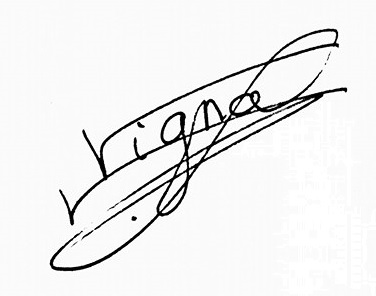
\includegraphics[scale=0.5]{images/Signature2.jpg}
    \end{figure}
    \begin{tabular}{c}
 \hrulefill \\
 Valentin Vignal \\
 \mydate\today\\
\end{tabular}
\end{center}
\newpage

% ####################################################################################################
% ####################################################################################################
% Acknowledgements
% ####################################################################################################
% ####################################################################################################

\begin{center}
    \textbf{\Large ACKNOWLEDGEMENTS}\\
\end{center}

I would like to express my special thanks or gratitude to my advisor Harold Soh who gave me the opportunity to work on this project combining Artificial Intelligence and Music.

Secondly I would also like to thanks all the member of the research team, and especially the PhD. students Abdul Fatir and Yaqi Xie who, despite their busy schedules, taught me, and help me in many scenarios.

I also yould like to thanks the Doctor Dorien Herremans who gave me precious advises at the beginning of my project.

\newpage
\tableofcontents
\newpage

% ####################################################################################################
% ####################################################################################################
% Summary
% ####################################################################################################
% ####################################################################################################

\setlength{\parindent}{0.6cm}

% ----- Specification -----
% The thesis must contain a summary of not more than 500 words written in the English Language. If prior approval from the Faculty has been obtained at the time of admission for a thesis to be written in a language other than English, it must contain a summary of not more than 500 words written in that language in addition to a summary not exceeding 500 words written in the English Language. The summary must be included in the thesis.

% \begin{center}
%     \textbf{\Large SUMMARY}
% \end{center}
\chapter*{Summary}
\addcontentsline{toc}{chapter}{Summary}      % To not display number of chapter in table of content

This paper introduces the work I have done for my dissertation.
As a musician, I like to play music, improvise and create or arrange songs.
The main goal of this dissertation is to create a neural network architecture able to handle all the tasks a musician or a composer can do.

To do so, I created a new architecture that I call RMVAE (Recurrent Multimodal Variational AutoEncoder) (section \ref{sec:rmvae}) which combines the MVAE architecture \cite{wu_multimodal_2018} and LSTM cells (see section \ref{sec:back:rnn}).
Only one trained model can be used to create a melody, several musical parts at the same time, harmonize a melody or reconstruct missing parts in a song.

As a musician I also tried to integrate prior musical knowledge to the model by creating 3 cost functions (section \ref{sec:loss}).

For this project, I used the MIDI dataset which is Bach's Chorales dataset from the music21 corpus \cite{noauthor_music21corpuschorales_nodate} and used their framework \cite{noauthor_music21_nodate} to open and create MIDI files.
The deep learning framework I used it Tensorflow/Keras \cite{noauthor_tensorflow_nodate, noauthor_keras_nodate}.
I made my python code for this dissertation available online: \url{https://github.com/ValentinVignal/midiGenerator}.

The results show that the extra losses are not helping the model which indicates that the neural network is able to understand those musical rules and tendencies by its own.

% ####################################################################################################
% ####################################################################################################
% List of Tables
% ####################################################################################################
% ####################################################################################################

\listoftables

% ####################################################################################################
% ####################################################################################################
% List of Figures
% ####################################################################################################
% ####################################################################################################

\listoffigures

% ####################################################################################################
% ####################################################################################################
% List of Illustration
% ####################################################################################################
% ####################################################################################################


% ####################################################################################################
% ####################################################################################################
% List of Syhmbols
% #####################################################################################################
% #####################################################################################################
\newpage
\begin{center}
    \textbf{\Large LIST OF SYMBOLS}\\
    \vspace{2cm}
    \begin{longtable}{ll}
        AE & Auto Encoder \\
        AI & Artificial Intelligence \\
        AMAE & ArgMax AutoEncoder \\
        C-RBM & Convolutional Restricted Boltzmann Machine \\
        CNN & Convolutional Neural Network \\
        FC & Fully Connected \\
        GAN & Generative Adversarial Network \\
        GRU & Gated Recurrent Unit \\
        KLD & Kullback-Leibler Divergence \\
        LSTM & Long Short-Term Memory \\
        MCMC & Markov Chain Monte Carlo \\
        MDMM & Multimodal Deep Markov Model \\
        MIDI & Musical Instrument Digital Interface \\
        ML & Machine Learning \\
        MVAE & Multimodal Variational AutoEncoder \\
        NADE & Neural Autoregressive Distribution Estimation \\
        NN & Neural Network \\
        PoE & Product of Experts \\
        RBM & Restricted Bolzmann Machine \\
        ReLU & Rectified Linear Unit \\
        RL & Reinforcement Learning \\
        RMVAE & Recurrent Multimodal Variational AutoEncoder \\
        RNN & Recurrent Neural Network \\
        RPoE & Recurrent Product of Experts \\
        RTRBM & Recurrent Temporal Restricted Boltzmann Machine \\
        SGD & Stochastic Gradient Descent \\
        VAE & Variational AutoEncoder \\
        VQ-VAE & Vectore Quantisation - Variational AutoEncoder \\
        VRAE & Variational Recurrent AutoEncoder \\
    \end{longtable}
    
\end{center}
\newpage

\pagenumbering{arabic}

% ####################################################################################################
% ####################################################################################################
% Main body of the thesis
% #####################################################################################################
% #####################################################################################################


% ----------------------------------------------------------------------------------------------------
% Introduction
% ----------------------------------------------------------------------------------------------------
\chapter{Introduction}
My Introduction

% ----------------------------------------------------------------------------------------------------
% Background
% ----------------------------------------------------------------------------------------------------
\chapter{Background}

In this chapter, I will introduce some background knowledge that might be useful to the reader. Since this project is about music generation, I will explain and illustrate some basic concepts about music.

I will consider the Western music using equal temperament and don't consider the inharmonicity of stringed instruments. These are common assumptions in all the existing works about music generation.

% -------------------- Music Representation --------------------

\section{Music representation}

In this section I will explain how musicians represent the music on paper, and from it, how it is possible to represent the music in a abstract way in a computer without encoding any waveforms or actual \textit{sounds}.

\subsection{Musical stave}

It is very useful for anyone to be able to write down their work to save it or share it with someone else. Musicians faced this issue too. They came up with the musical stave :

\begin{figure}[H]
    \centering
    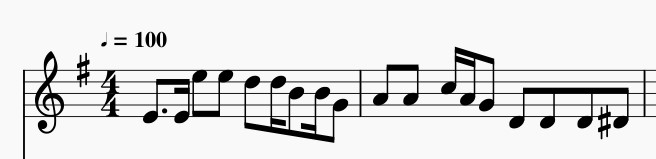
\includegraphics[scale=0.75]{images/music/stave/musical_stave_example.jpg}
    \caption{Musical Stave example}
    \label{fig:musical_stave_example}
\end{figure}

The vertical axis is the frequency axis an the horizontal axis corresponds to the time axis.
In the figure \ref{fig:musical_stave_example}, it is written that the tempo is $100 BPM$, the scale is \textit{G major} (one \musSharp) and the measure are divided with 4 beats ($4/4$ inscription).
As said previously, the vertical position of a note indicates its frequency :

\begin{figure}[H]
   \begin{minipage}{0.5\textwidth}
     \centering
     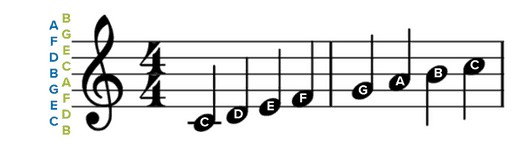
\includegraphics[width=.9\linewidth]{images/music/stave/note_names.jpg}
     \caption{Notes on a musical stave}
     \label{fig:note_names}
   \end{minipage}\hfill
   \begin{minipage}{0.5\textwidth}
     \centering
     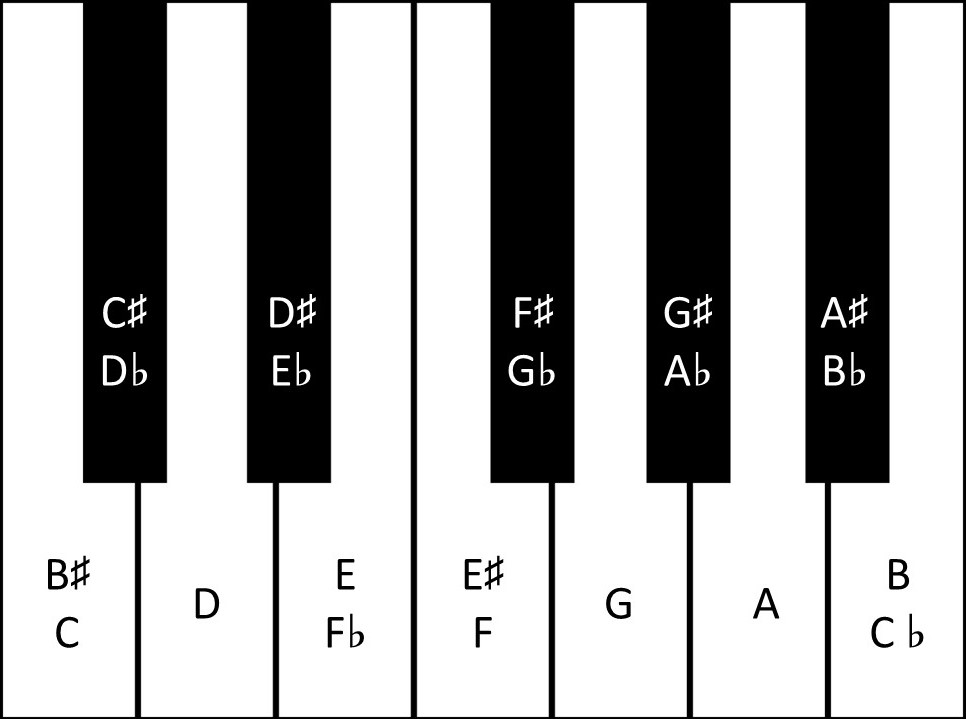
\includegraphics[width=.9\linewidth]{images/music/piano/piano_keys.jpg}
     \caption{Notes on Piano}
     \label{fig:piano_keys}
   \end{minipage}
\end{figure}

The figures \ref{fig:note_names} and \ref{fig:piano_keys} show the correspondence between the notes on a musical stave and on a piano keyboard. By default the notes correspond to the white keys of the piano (it is the C major scale).

One thing to know is that, between 2 followings notes (or piano keys, including white and black keys), the ratio between the fundamental frequencies of the 2 notes is always equal to $\sqrt{12}$. It means that if we consider the notes $A4$ and $A5$ (2 $A$ notes in the octaves 4 and 5), the ratio between the fundamental frequencies is $2$. This information will help to understand chords construction.

The length of a note is defined by its shape as shown in the Table \ref{tab:notes_duration}. This table is describing the relation between the length of a note, and its shape on the musical stave.

\begin{table} [ht]
    \begin{center}
        \begin{tabular} {c|c|c}
            Name & Duration & Symbol \\
            \hline
            Whole note & $4$ beats & {\Large \musWhole} \\ 
            Half note & $2$ beats & {\Large \musHalf} \\
            Quarter note & $1$ beat & {\Large \musQuarter} \\
            Eighth note & $1/2$ beat & {\Large \musEighth} \\
            Sixteenth note & $1/4$ beat & {\Large \musSixteenth} \\
        \end{tabular}
        \caption{Note names and duration}
        \label{tab:notes_duration}
    \end{center}
\end{table}

In this work, we won't consider shorter notes than Sixteenth notes because most of the songs are not using them. This is a common assumption in the existing work.


\subsection{MIDI}
\label{sec:midi}

% The \textit{MIDI} format ($.mid$) is a format to save music as a file. However, it doesn't save the actual \textit{sound} of it. The way it works is very similar to the representation of a musical stave.

% In a midi file is a set of instructions. It will save for each instruments, for each notes (pitch) the times when the note starts and ends and some other information (like the velocity et caetera).

% To read a midi file, the computer has a collection of sound for every instruments, notes, velocity et caetera, and plays these sounds depending of the instructions read in the file.

\textit{MIDI} format ($.mid$) is a technical standard that describes a protocol.
It was first used to carry musical messages between electronic instruments, software and devices. These messages are events about note information (for example, pitch, velocity, panning...) an some other parameters (for example, vibrato, volume...). 
The to most important messages I will consider are:
\begin{itemize}
    \item \textit{Note on} is indicating that a note has to be played. It contains the channel information (which can be considered as an instrument), the pitch information (what note should be played) and the velocity. We could right an event as follow :
    \begin{equation}
        <NoteOn, 0, 50, 127>
    \end{equation}
    To describe the event \textit{Start to play the note $D3$ with the maximum velocity (127) for the channel (instrument) 0}
    \item \textit{Note off} is indicating to stop playing a note (for instance, release the keyboard key). The given parameters are the same as the ones given to the \textit{Note On} event.
    \begin{equation}
        <NoteOff, 0, 50, 127>
    \end{equation}
    will stop the note started with the previous \textit{Note On} event.
\end{itemize}

Each note is associated with a time value which can be expressed in number of ticks (time division). The header of file specifies how may ticks there are per quarter note.

\subsection{Pianoroll}

The pianoroll is a common representation of a musical stale in the music production softwares.

\begin{figure}[H]
    \centering
    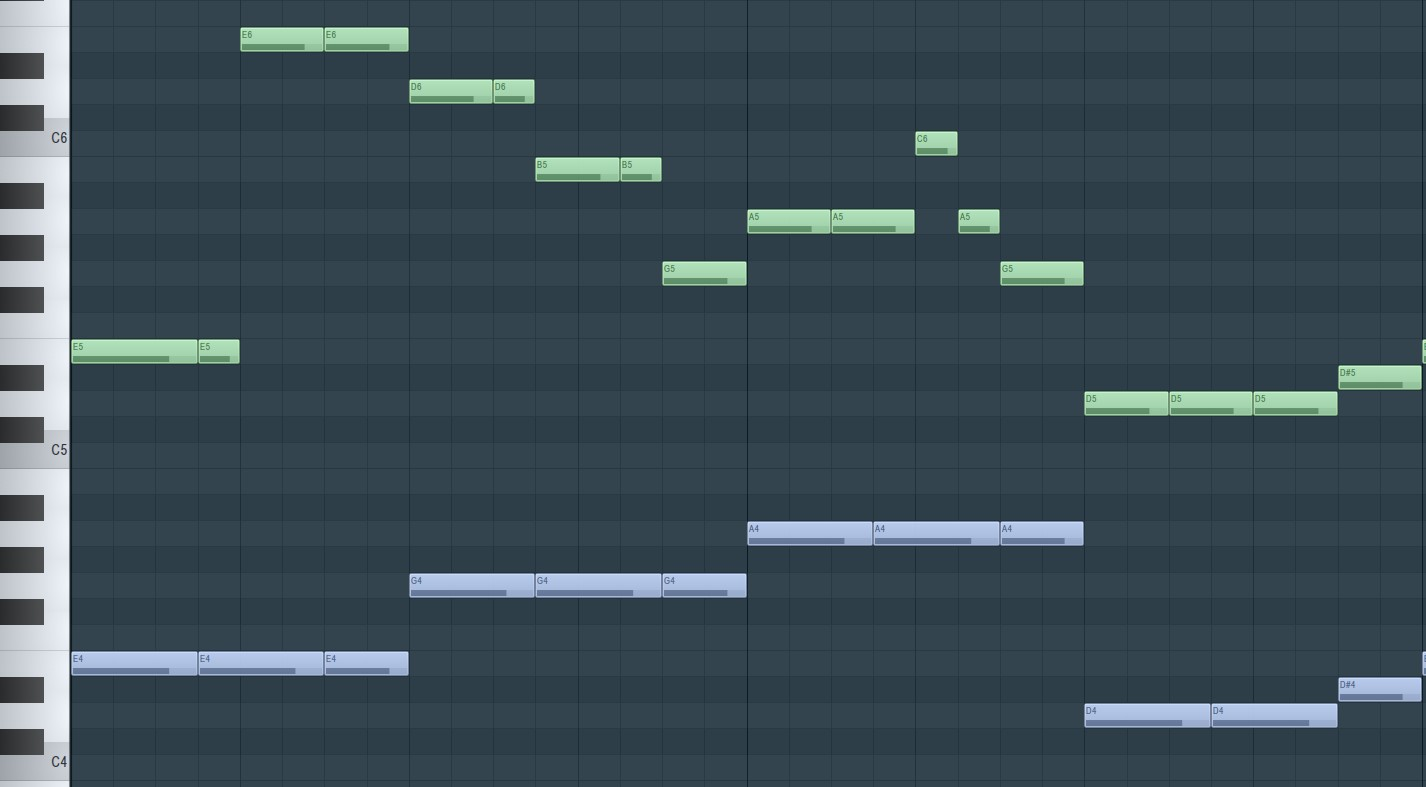
\includegraphics[width=0.75 \textwidth]{images/music/pianoroll/pianoroll_flstudio.jpg}
    \caption{Pianoroll example from the software FL Studio \cite{noauthor_fl_nodate}}
    \label{fig:pianoroll_flstudio}
\end{figure}

The figure \ref{fig:pianoroll_flstudio} shows a view of the pianoroll in the famous software \textit{FL Studio} \cite{noauthor_fl_nodate}. The composers of electronic music like EDM, Techno et caetera use this view to compose and arrange their songs.

% -------------------- Music Theory --------------------

\section{Music theory}

In this section, I will describe and explain some rules from the music theory which are related to this work. The rules I am going to explain about are the most common ones and most of the songs tend to follow them.

\subsection{Scale and Rhythm}

\subsubsection{Scale}

A \textit{scale} is a set of notes. Because the human ear is now used to it, the notes of a scale will sound nice when they are played together. In traditional Western music, it generally consists of 7 notes. They are several types of scales.
The most common is the \textit{Major scale} or the \textit{Natural Minor Scale}. For example, the C Major scale uses all the white keys of the piano (Figure \ref{fig:piano_keys}: A, B, C, D, E, F and G), as well as the A Natural Minor scale.

Another type of scales often used by the musicians to creates their \textit{solos} are the \textit{Pentatonic} scales.


\begin{figure}[H]
    \centering
    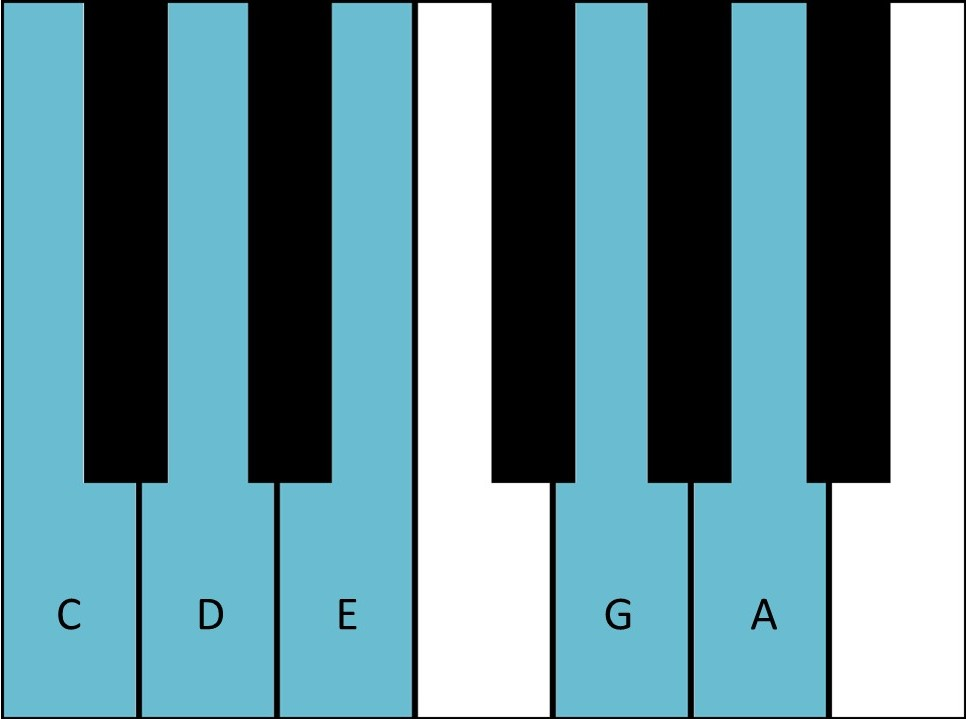
\includegraphics[width=0.5 \textwidth]{images/music/piano/pentatonic_scale.jpg}
    \caption{C Major Pentatonic scale (or A Minor Pentatonic scale)}
    \label{fig:pentatonic_scale_piano}
\end{figure}

As seen in the figure \ref{fig:pentatonic_scale_piano}, the C Major pentatonic scale (which uses the same notes as the A Minor pentatonic scale) uses only five notes (A, C, D, E and G) which are contained in the C Major Scale. It is known that playing in this scale will easily produce enjoyable and in-tune melodies or any musical parts. 


\subsubsection{Rhythm}

The rhythm is an important part of the current music like \textit{Pop Music}. It has the tendency to remain consistent through the song and to repeat some patterns.
It helps the listener to easily follow the progression and allows him to listen what he's expecting to.

However, rhythm is more flexible than scale and harmonies, and there is no rhythm theory someone could follow.
This is why classical music is not considered as a rhythmic music.

I this work, I considered and will consider only binary rhythm (each beat is divided into 2 smaller equal beats) and not ternary rhythm (each beat is divided into 3 smaller equal beats) because the binary rhythm is the most common one.


\subsection{Harmonics}
\label{sec:harmonics}

In this section, I will introduce some physical concept about musical sounds and timbre and then illustrate how it can explain some musical rules.

\subsubsection{Harmonics}

A sound is a sum of harmonics:

\begin{equation}
    s(t) = \sum_{n=1}^{\infty} \alpha_{n} \sin(n f t + \phi_{n})
\end{equation}
where $f$ is the fundamental frequency and $\phi$ the phase.

Let's take an example with the $A4$ note which has a its fundamental frequency equals to $440 Hz$.
Then the $2^{nd}$ harmonic is $A5$ $880Hz$.
The consequence is , when an instrument plays a $A4$, all the harmonics of a $A5$ are also present.
Let us take one step further, the $3^{rd}$ harmonic of $A4$ is $E5$ $1320Hz$. It means it is possible to hear a $E5$ from a played $A4$.
The table \ref{tab:A4_harmonics} is referencing the firsts harmonics of the $A4$ note.

\begin{table} [ht]
    \begin{center}
        \begin{tabular} {c||c|c|c}
            Harmonic number & Frequency ($Hz$) & Note Name & Musical Interval \\
            \hline
            $1$ & $440$ & $A4$ & Unison \\
            $2$ & $880$ & $A5$ & Octave \\
            $3$ & $1320$ & $E5$ & Fifth \\
            $4$ & $1760$ & $A6$ & Octave \\
            $5$ & $2200$ & $C\sh6$ & Major Third \\
            $6$ & $2640$ & $E6$ & Fifth \\
        \end{tabular}
        \caption{Harmonics of $A4$}
        \label{tab:A4_harmonics}
    \end{center}
\end{table}

From the table \ref{tab:A4_harmonics}, we can notice:
\begin{itemize}
    \item The $A$ and $E$ notes are linked together (\textit{Fifth} or reversed \textit{Fourth} interval).
    \item The $A$ and $C\sh$ notes are linked together (\textit{Major Third} interval).
\end{itemize}


\subsubsection{Chords}

The links between notes illustrated in the table \ref{tab:A4_harmonics} explains why a Major chord sound \textit{nice} or \textit{smooth}.
A $A$ $Major$ chord is composed with 3 notes : $A$, $C\sh$ and $E$. All the notes are already contained in the harmonics of a $A$ sound.

A Minor chords ($A$ $Minor$ is $A$, $C$, $E$) will also sounds acceptable to the human ears because $A$ and $C$ share $E$ in their harmonics (respectively the \textit{Fifth} interval and \textit{Third Major} interval) 

\subsubsection{Dissonance}

When 2 frequencies are close to each other and added up, it is possible to observe a resonance phenomena:

\begin{figure}[H]
    \centering
    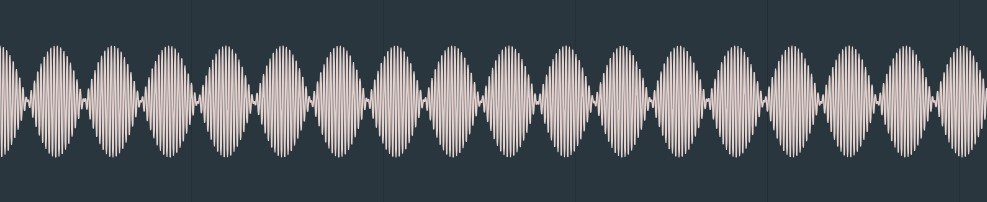
\includegraphics[width=\textwidth]{images/music/waveform/resonance.jpg}
    \caption{Resonance waveform}
    \label{fig:resonance}
\end{figure}
The figure \ref{fig:resonance} shows the waveform generated by a $B4$ ($494Hz$) and a $C5$ ($523Hz$) (\textit{semitone} interval).
This phenomena is explained by the trigonometric identity:

\begin{equation}
    \cos(f) + \cos(f + \delta f) = 2 \cos(\frac{2f + \delta f}{2}) \cos(\frac{\delta f}{2})
\end{equation}

This phenomena is unpleasant to hear and this is why, musician usually try to avoid to play notes that generate a resonance between their harmonics:
\begin{itemize}
    \item \textit{Semitone} interval (ex: $A$ and $A\sh$)
    \item \textit{Tone} interval (ex: $A$ and $B$)
    \item \textit{Tritone} interval (ex: $A$ and $D\sh$)
\end{itemize}


\subsubsection{Harmony}

Either for classical music (Bach Chorales) or pop music (back singers), a common method to \textit{fill a song} is to add harmony parts to the lead melody. The harmony parts usually follow the lead melody but on other notes.
An example is provided in the figure \ref{fig:harmony_example}.

\begin{figure}[H]
    \centering
    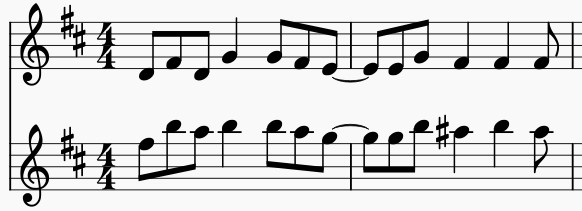
\includegraphics[width=0.75 \textwidth]{images/music/stave/harmony.jpg}
    \caption{Lead voice and its harmony part}
    \label{fig:harmony_example}
\end{figure}

The harmony parts will usually avoid unpleasant interval and mostly try to create the following ones: 
\begin{itemize}
    \item \textit{Octave} and \textit{unison} interval
    \item \textit{Fifth} interval
    \item \textit{Fourth} interval
    \item \textit{Major Third} interval
    \item \textit{Minor Third} interval
\end{itemize}


% -------------------- Music arrangement  --------------------

\section{Music arrangement}

Arranging a song is an entire musical field an a job.
It is the art of giving an existing melody musical variety.
To put it more simply, it is creating a accompaniment for an melody.
I can includes chords, change the rhythm, add other musical parts.

To give an example, arranging a song could be create a piano/guitar/drums/bass parts from lyrics and a voice melody.


% -------------------- Neural Network architecture --------------------

\section{Neural Network architectures}

In this section, I will briefly describe some neural network architectures.

\subsection{Convolutional neural network}

The convolutional networks are often used on images because they can preserve the spatial information.
A CNN usually includes two types of layers :
\begin{itemize}
    \item A convolutional layer
    \item A pooling layer
\end{itemize}

\subsubsection{Convolutional Layer}

For a 2D convolution, the convolutional layer which takes as input a tensor of shape \texttt{(height, width, channels)}.
The \textit{filter} of the convolutional layer will have a shape \texttt{(h, w, channels)}.
Then the layer will do a $2D$ convolutional operation between the filter and the input through the axes corresponding to the \texttt{height} and the \texttt{width}.

\begin{equation}
    y_{\tau} = \sum_{t=0}^{l-1} w_{t} \times x_{\tau + t}
    \label{eq:convo}
\end{equation}

The equation \ref{eq:convo} shows the mathematical transformation for a 1D convolution with $x$ as the input, $w$ as the filter/kernel and $y$ as the output.

\subsubsection{Pooling Layer}

A pooling layer is used to reduce the size of a tensor. It extracts a value from a region of the tensor. Two common poolings are:
\begin{itemize}
    \item The \textit{Average pooling} which takes the average of the region
    \item The \textit{Max pooling} which takes the maximum of the region
\end{itemize}
The figure \ref{fig:max_pooling} illustrates how the max pooling operation works.

\begin{figure}[H]
    \centering
    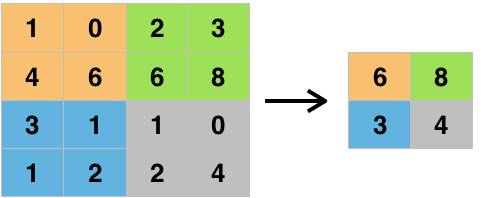
\includegraphics[width=0.75 \textwidth]{images/nn/layers/max_pooling.png}
    \caption{Max pooling operation}
    Source: \href{https://en.wikipedia.org/wiki/File:Max_pooling.png}{Wikipedia}
    \label{fig:max_pooling}
\end{figure}

\subsection{AutoEncoder}
\label{sec:back:ae}

An AE \cite{moor_topological_2020, tschannen_recent_2018, rudolph_structuring_2019} is composed of a \textit{encoder} and a \textit{decoder}.
First, the input goes into the encoder.
The output of the encoder is the latent space (the hidden layers), which is smaller than the input.
The output of the encoder becomes the input of the decoder.
The goal of the decoder is to reconstruct the input from the latent space.
The hidden layers of the AE are smaller than the input which forces the network to compress the input and reduce its dimensions.
Therefor, the AE has to learn "high level features" about the inputs.
The figure \ref{fig:autoencoder} summarizes this architecture.

\begin{figure}[H]
    \centering
    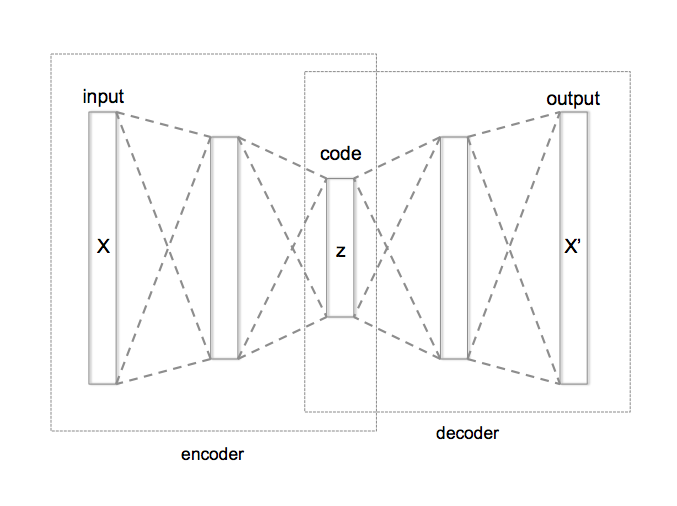
\includegraphics[width=0.75 \textwidth]{images/nn/architectures/autoencoder.png}
    \caption{AutoEncoder}
    Source: \href{https://commons.wikimedia.org/wiki/File:Autoencoder_structure.png}{Wikipedia}
    \label{fig:autoencoder}
\end{figure}

\subsection{Variational AutoEncoder}
\label{sec:back:vae}

A VAE \cite{doersch_tutorial_2016, noauthor_variational_nodate, noauthor_tutorial_nodate, akrami_robust_2019, liu_towards_2020} is an autoencoder. The steps are the following:
\begin{enumerate}
    \item The input goes first in the encoder which encodes it as a gaussian distribution over the latent space.
    \item A point is sample from this distribution.
    \item This point is decoder by the decoder to reconstruct the input.
\end{enumerate}

By encoding the normal distribution and not directly the latent space, it is possible to regularize the output of the encoder to avoid overfitting and ensure that the latent space as good properties that enable generative process.

To regularize the output of the decoder, an extra term is added to the loss function : Kulback-Leibler Divergence (KLD) between the encoded distribution and the centred and reduced normal distribution :

\begin{equation}
    \mathbb{D}_{KL} (\mathcal{N}(\mu_{encoded}, \sigma_{encoded}), \mathcal{N}(0, 1))
\end{equation}

\subsection{Generative Adversarial Network}
\label{sec:back:gan}

GAN \cite{noauthor_gan_2017, goodfellow_generative_2016, goodfellow_generative_2014} are composed of two models that are trained simultaneously:
\begin{itemize}
    \item The \textit{Generator} will learn how to create data that look real
    \item The \textit{Discriminator} will learn how to differentiate real and generated data.
\end{itemize}

The discriminator is trained with real data and data generated by the generator. The goal of the discriminator is to classify the real data as \textit{"Real"} and the generated data as \textit{"Fake"}.
On the other side, the generator takes some noise as an input to generate a datum.
Its goal is to make the discriminator classify its generated data as \textit{"Real"}.

Through training, the generator will get better and create more consistent data so the discriminator classify them as Real.
It will then for the the discriminator to get better and classify real and fake data more precisely.
Thus, the generator is forced to create data which look more real.
And so on...

\subsection{Recurrent Neural Networks}
\label{sec:back:rnn}

A RNN is a neural network where connections between nodes form a direct graph along a temporal sequence. The general architecture is showed in the figure \ref{fig:rnn}.

\begin{figure}[htbp]
    \centering
    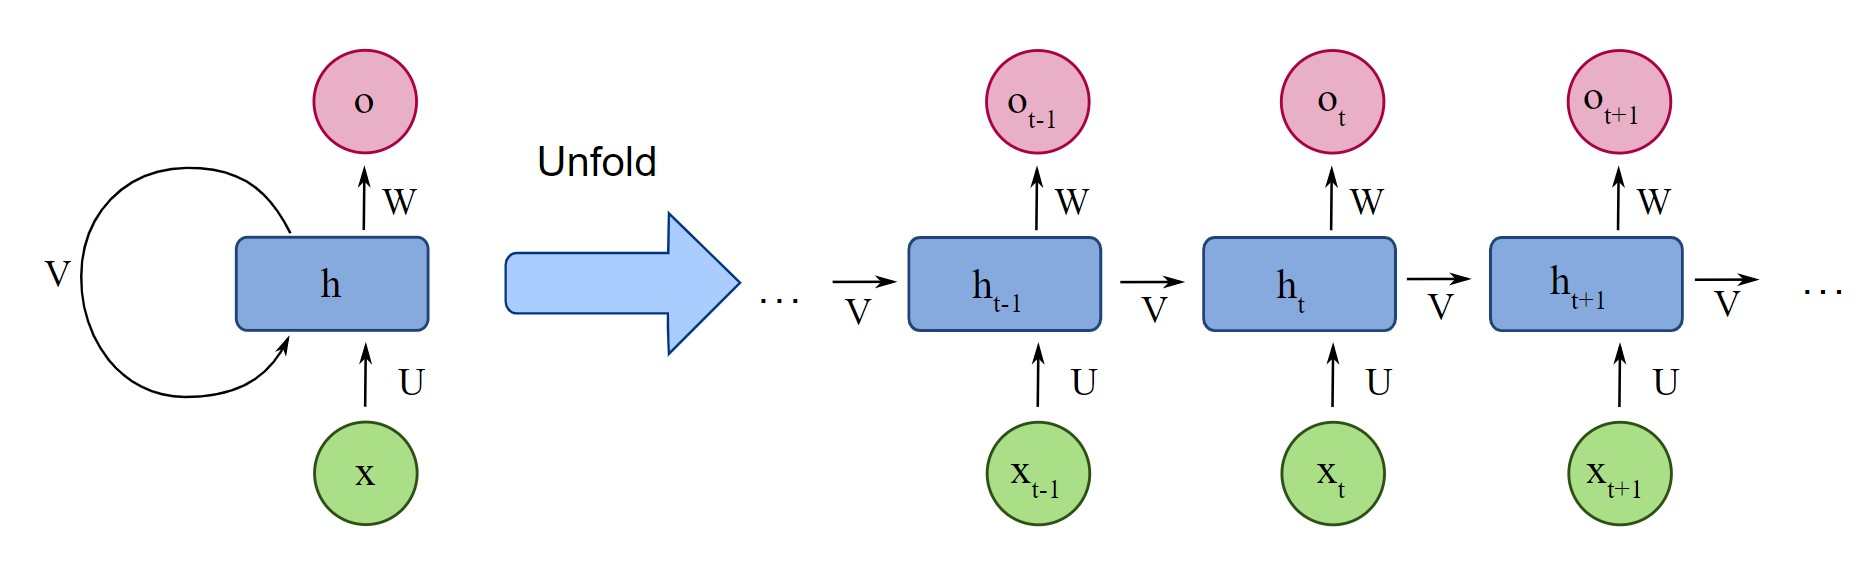
\includegraphics[width=0.75 \textwidth]{images/nn/architectures/rnn.jpg}
    \caption{Recurrent Neural Network}
    Source: \href{https://fr.wikipedia.org/wiki/Fichier:Recurrent_neural_network_unfold.svg}{Wikipedia}
    \label{fig:rnn}
\end{figure}

The most used cells used are the LSTM cell and the GRU cell. The architectures are showed in the figures \ref{fig:lstm} and \ref{fig:gru}.

\begin{figure}[htbp]
   \begin{minipage}{0.5\textwidth}
     \centering
     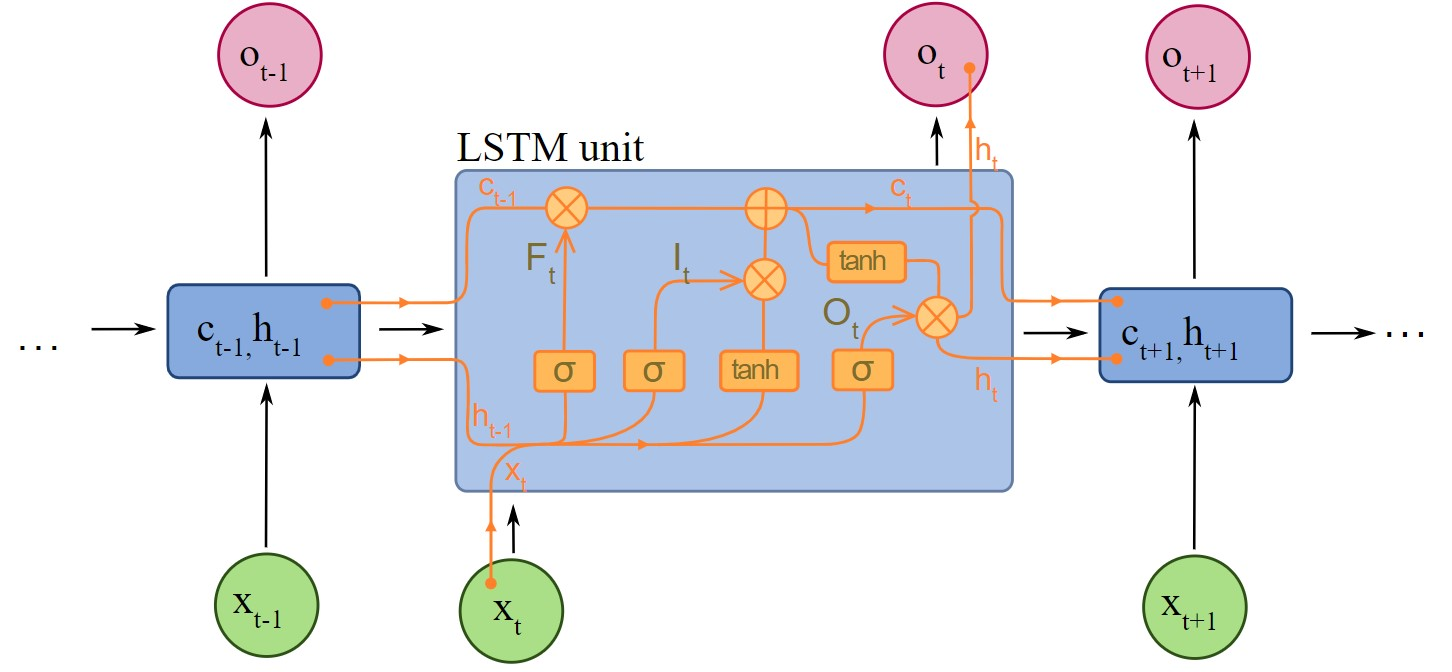
\includegraphics[width=.95\linewidth]{images/nn/layers/lstm.jpg}
     \caption{LSTM cell}
     Source: \href{https://commons.wikimedia.org/wiki/File:Long_Short-Term_Memory.svg}{Wikipedia}
     \label{fig:lstm}
   \end{minipage}\hfill
   \begin{minipage}{0.5\textwidth}
     \centering
     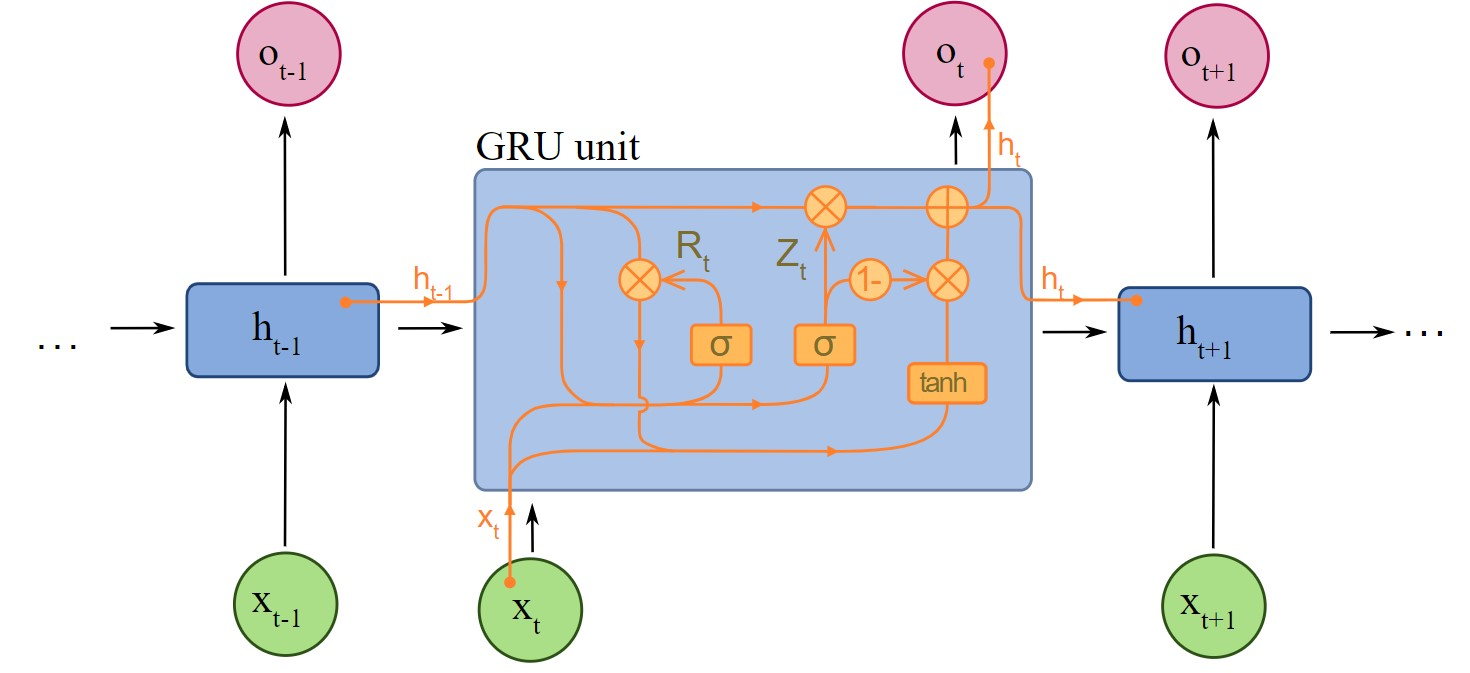
\includegraphics[width=.95\linewidth]{images/nn/layers/gru.jpg}
     \caption{GRU cell}
     Source: \href{https://en.wikipedia.org/wiki/Recurrent_neural_network#/media/File:Gated_Recurrent_Unit.svg}{Wikipedia}
     \label{fig:gru}
   \end{minipage}
\end{figure}


\subsection{Transformers}
\label{sec:back:transformers}

The Transformers \cite{vaswani_attention_2017, noauthor_transformer_nodate, giacaglia_transformers_2019, allard_what_2020, alammar_illustrated_nodate} have be introduced to the world by Ashish Vaswani et al. \cite{vaswani_attention_2017-1}.
It is an attention mechanism illustrated in the figure \ref{fig:arch:transformer}.
On this figure, the encoder is on the left and the decoder on the right.

The scaled dot-product attention and multi-head attention layers are drawn in the figures \ref{fig:scaled_dot_product_attention} and \ref{fig:multi_head_attention}.

\begin{figure}[htbp]
    \centering
    \newlength{\MyOtherHeightFour}
    \settoheight{\MyOtherHeightFour}{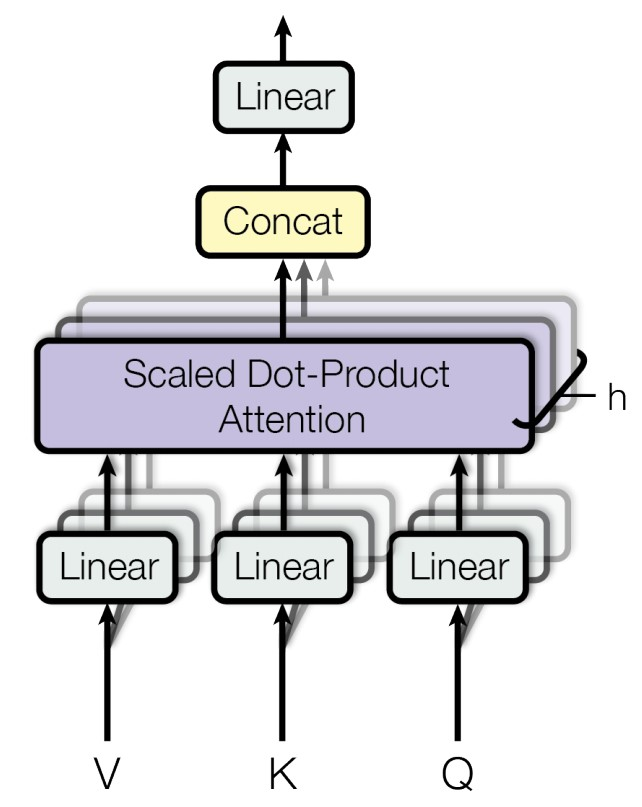
\includegraphics[width=0.9 \textwidth]{images/related_works/transformer/multi_head_attention.jpg}}
    \begin{subfigure}[t]{0.49\textwidth}
        \centering
        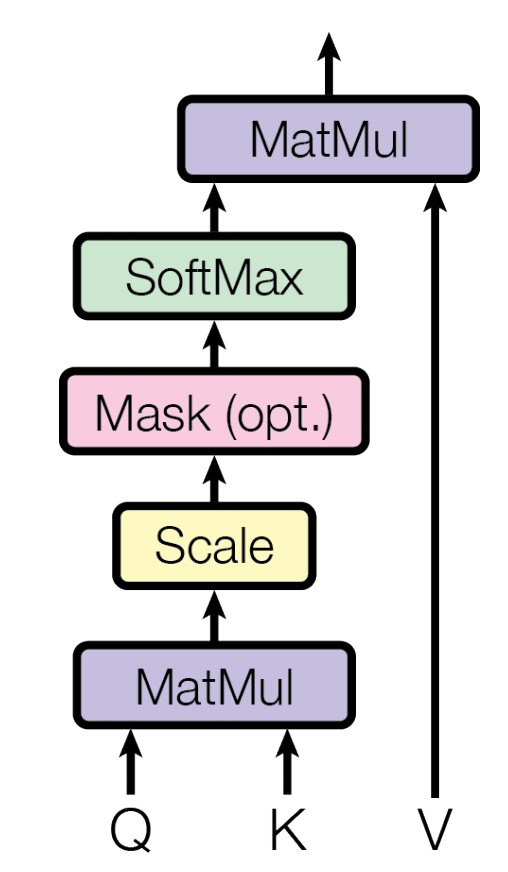
\includegraphics[width=.6\textwidth]{images/related_works/transformer/scaled_dot_product_attention.jpg}
        \caption{Scaled Dot-Product Attention}
        Source: Ashish Vaswani et al.'s paper \cite{vaswani_attention_2017-1}
        \label{fig:scaled_dot_product_attention}
    \end{subfigure}
    \hfill
    \begin{subfigure}[t]{0.49\textwidth}
        \centering
        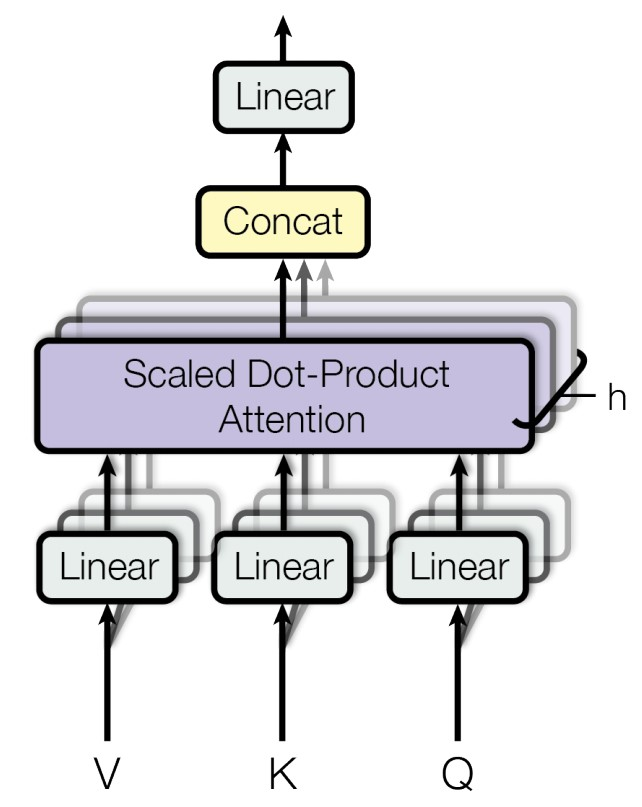
\includegraphics[width=.9 \textwidth]{images/related_works/transformer/multi_head_attention.jpg}
        \caption{Multi-Head Attention}
        Source: Ashish Vaswani et al.'s paper \cite{vaswani_attention_2017-1}
        \label{fig:multi_head_attention}
    \end{subfigure}
    \caption{Scaled Dot-Product Attention and Multi-Head Attention}
    Source: Ashish Vaswani et al.'s paper \cite{vaswani_attention_2017-1}
    \label{fig:arch:attention}
\end{figure}

The scaled dot-product attention operation is the follows the equation \ref{eq:scaled_dot_product_attention}.
\begin{equation}
    \text{Attention} (Q, K, V) = \text{softmax}(\frac{QK^T}{\sqrt{d_k}})V
    \label{eq:scaled_dot_product_attention}
\end{equation}
where $d_k$ is the number of dimensions.

And the multi-head attention operation follows the the equation \ref{eq:multi_head_attention}.
\begin{equation}
    \text{MultiHead}(Q, K, V) = \text{Concat}(\text{head}_1, \dots, \text{head}_d) W^O
    \label{eq:multi_head_attention}
\end{equation}
where $\text{head}_i = \text{Attention}(QW_i^Q, KW_i^K, VW_i^V)$.

To summarise the process, Q, K and V are respectively called the queries, the keys and the values.
Their attention function can be described as mapping a query and a set of key-value pairs to an output, where the query, keys, values, and output are all vectors.
The output is computed as a weighted sum of the values, where the weight assigned to each value is computed by a compatibility function of the query with the corresponding key.

The advantage of the transformer is that it is able to learn long-range dependencies.
This is a challenge in many sequences tasks.
However, a transformer doesn't take into account the position of the input from a sequence. 
Therefor, a positional encoding must be added.

\subsection{Multimodel Variational AutoEncoder}
\label{sec:back:mvae}

The MVAE has been introducted by Mike Wu et al. \cite{wu_multimodal_2018}.
The figure \ref{fig:mvae_graph} represent the graphical model of the MVAE.
The gray circles represent the observed variables.
The MVAE uses a \textit{Product of Experts} (PoE) inference network and a sub-sampled training paradigm to solve the multi-modal inference problem.

% Good example how to use tikz:
% https://tex.stackexchange.com/questions/193694/drawing-graph-of-markov-chain-with-patches-using-tikz
\begin{figure}[htbp]
\begin{center}
    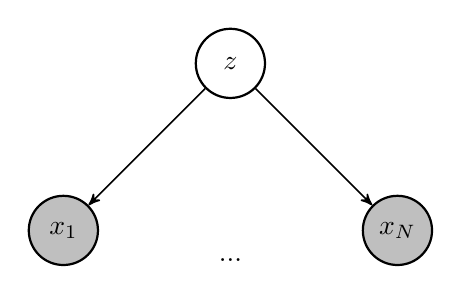
\begin{tikzpicture}[->, >=stealth', auto, semithick, node distance=3cm]
    \tikzstyle{every state}=[fill=white,draw=black,thick,text=black,scale=1]
    \node[state](z){$z$};
    \node[state, fill=lightgray](x1)[below left of=z]{$x_1$};
    \node[above=0.5cm](dots)[below of=z]{$...$};
    \node[state, fill=lightgray](xn)[below right of=z]{$x_N$};
    \path
        (z) edge    node{}    (x1)
            edge    node{}    (xn);
    \end{tikzpicture}
\caption{Graphical model of the MVAE}
\label{fig:mvae_graph}
\end{center}
\end{figure}


The conditional independence assumptions in the generative model (figure \ref{fig:mvae_graph}) imply a relation among joint- and single-modality posteriors :

\begin{equation}
    \begin{split}
        p(z|x_1, ..., x_N) & = \frac{p(x_1, ..., x_N | z) p(z)}{p(x_1, ..., x_N)} \\
        & = \frac{p(z)}{p(x_1, ..., x_N)} \prod_{i=1}^{N} p(x_i | z) \\
        & = \frac{p(z)}{p(x_1, ... x_N)} \prod_{i=1}^{N} \frac{p(z|x_i)p(x_i)}{p(z)} \\
        & = \frac{\prod_{i=1}^{N} p(z|x_i)}{\prod_{i=1}^{N-1} p(z)} \frac{\prod_{i=1}^{N}p(x_i)}{p(x_1, ..., x_N)} \\
        & \propto \frac{\prod_{i=1}^{N} p(z|x_i)}{\prod_{i=1}^{N-1} p(z)}
        \approx \frac{\prod_{i=1}^{N} (\widetilde{q}(z|x_i)p(z))}{\prod_{i=1}^{N-1} p(z)}
        = p(z) \prod_{i=1}^{N} \widetilde{q}(z | x_i) \\
        & \text{With $\widetilde{q}(z|x_i)$ the model approximation of $\frac{p(z|x_i)}{p(z)}$}
    \label{eq:poe}
    \end{split}
\end{equation}

The PoE can be used , including a \textit{“prior expert”}, as the approximating distribution for the joint-posterior.

\begin{figure}[h]
    \centering
    \newlength{\MyOtherHeight}
    \settoheight{\MyOtherHeight}{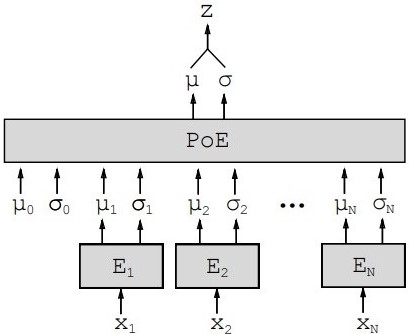
\includegraphics[width=0.9 \textwidth]{images/nn/architectures/mvae_all.jpg}}
    \begin{subfigure}[t]{0.49\textwidth}
        \centering
        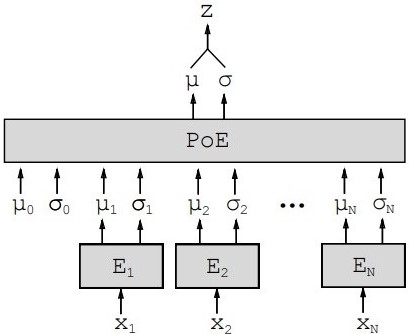
\includegraphics[width=.9 \textwidth]{images/nn/architectures/mvae_all.jpg}
        \caption{With all the modalities}
        \label{fig:mvae_architecture_all}
    \end{subfigure}
    \hfill
    \begin{subfigure}[t]{0.49\textwidth}
        \centering
        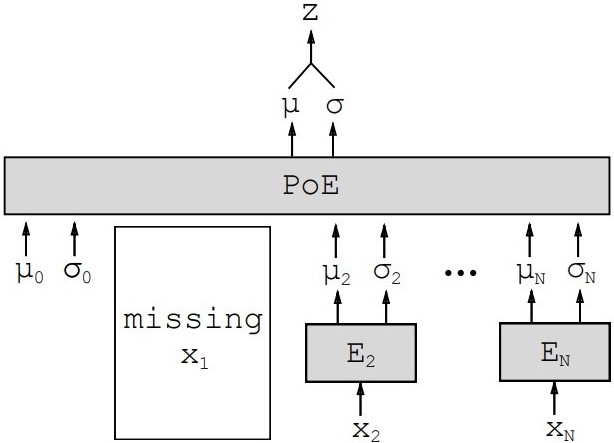
\includegraphics[width=.9 \textwidth]{images/nn/architectures/mvae_missing.jpg}
        \caption{With missing modalities}
        \label{fig:mvae_architecture_missing}
    \end{subfigure}
    \caption{MVAE architecture}
    Source: Mike Wu's paper \cite{wu_multimodal_2018}.
    \label{fig:mvae_architecture}
\end{figure}

The figure \ref{fig:mvae_architecture} shows how the PoE can handle missing modalities by simply ignoring them.

\subsection{Muldimodal Deep Markov Model}
\label{sec:back:mdmm}

% TODO: Explain MDMM

\subsection{Neural Autoregressive Distribution Estimation}
\label{sec:back:nade}

A NADE \cite{uria_neural_2016, uria_deep_2014} is a neural network made to support a $D$-dimensional distribution $p(x)$ which verify:
\begin{equation}
    p(x) = \prod_{d=1}^{D} p(x_{o_{d}} | x_{o_{<d}})
\end{equation}

It is a feed forward network parameterized as follow:
\begin{equation}
    p(x_{o_{d}} = 1 | x_{o_{<d}}) = \text{sigm}(V_{o_{d}, .} h_{d} + b_{o_{d}})
\end{equation}
\begin{equation}
    h_d = \text{sigm}(W_{., o_{<d}} x_{o_{<d}} + c)
\end{equation}
where, with $H$ as the number of hidden units, $V \in \mathbb{R}^{D \times R}$, $b \in \mathbb{R}^{D}$, $W \in \mathbb{R}^{H \times D}$, $c \in \mathbb{R}^{H}$.

The hidden matrix $W$ and bias $c$ are shared by each hidden layer $h_{d}$.
\begin{figure}[ht]
    \centering
    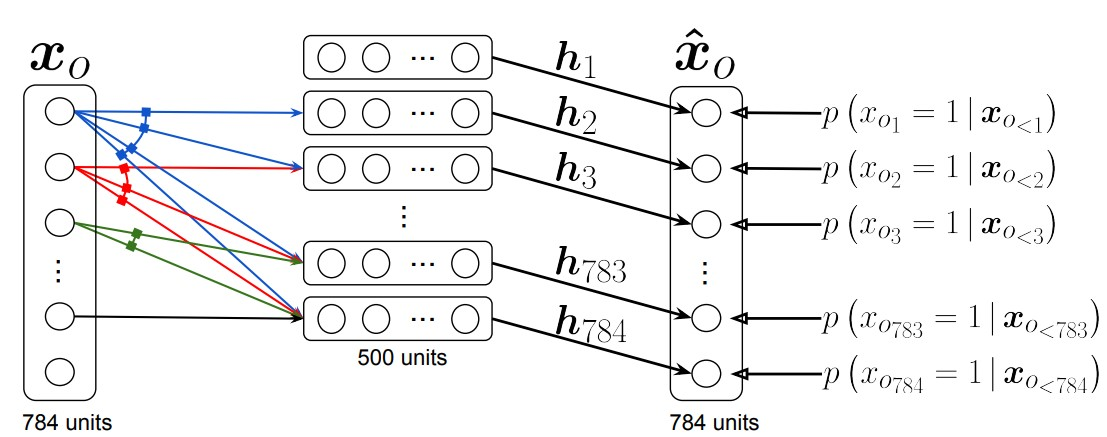
\includegraphics[width=0.75 \textwidth]{images/nn/architectures/nade_architecture.jpg}
    \caption{NADE architectue}
    Source: Benigno Uria et al.'s paper \cite{uria_neural_2016}
    \label{fig:arch:nade}
\end{figure}
The figure \ref{fig:arch:nade} illustrates the Nade model.
There is no path of connections between an output and the value being predicted, or element $x_O$ later in the ordering.
Arrows connected together correspond to connections with shared (tied) parameters.

\subsection{Restricted Bolzmann Machine}
\label{sec:back:rbm}

A RBM is an undirected graphical model \cite{noauthor_restricted_2018, montufar_restricted_2018, salakhutdinov_restricted_2007, fischer_introduction_2012} showed in the figure \ref{fig:arch:rbm}.
As an AE, it encodes the input $x$ in a latent space $h$ where:
\begin{equation}
    h_{i} = \text{sigmoid}(x^{T} W_{i} + a)
\end{equation}
where $x$ is the input, $h$ is the vector corresponding to the hidden layer, $W$ are the weights, $a$ is the hidden layer bias vector.
This is the endoding phase.

For the decoding, or reconstruction phase, the predicted output by the model is:
\begin{equation}
    x^{*}_{i} = \text{sigmoid}(h W^{T} + b)
\end{equation}
where $x^{*}$ is the reconstructed input, $W$ are the same weights as the forward pass, and $b$ are the observed layer bias vector.

\begin{figure}[htbp]
    \centering
    \begin{subfigure}[t]{0.49\textwidth}
        \begin{center}
            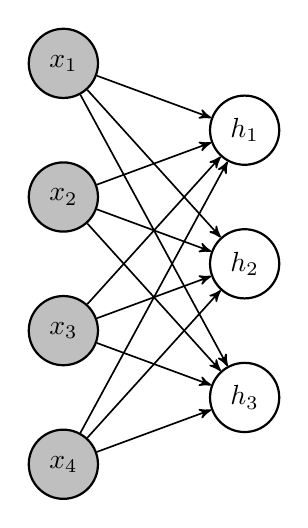
\begin{tikzpicture}[->, >=stealth', auto, semithick, node distance=1.2cm]
            \tikzstyle{every state}=[fill=white,draw=black,thick,text=black,scale=1]
            \node[state, fill=lightgray](x1)[left=1cm]{$x_1$};
            \node[state](h1)[below right of=x1, right=1cm]{$h_1$};
            \node[state, fill=lightgray](x2)[below left of=h1, left=1cm]{$x_2$};
            \node[state](h2)[below right of=x2, right=1cm]{$h_2$};
            \node[state, fill=lightgray](x3)[below left of=h2, left=1cm]{$x_3$};
            \node[state](h3)[below right of=x3, right=1cm]{$h_3$};
            \node[state, fill=lightgray](x4)[below left of=h3, left=1cm]{$x_4$};
            
            \draw (x1) -> (h1);
            \draw (x2) -> (h1);
            \draw (x3) -> (h1);
            \draw (x4) -> (h1);
            \draw (x1) -> (h2);
            \draw (x2) -> (h2);
            \draw (x3) -> (h2);
            \draw (x4) -> (h2);
            \draw (x1) -> (h3);
            \draw (x2) -> (h3);
            \draw (x3) -> (h3);
            \draw (x4) -> (h3);
            \end{tikzpicture}
        \end{center}
        \caption{RBM forward pass}
        \label{fig:rmb_forward}
    \end{subfigure}
    \begin{subfigure}[t]{0.49\textwidth}
        \begin{center}
            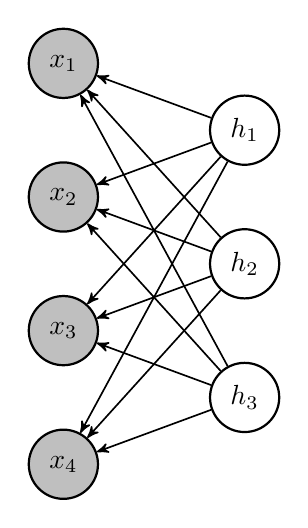
\begin{tikzpicture}[->, >=stealth', auto, semithick, node distance=1.2cm]
            \tikzstyle{every state}=[fill=white,draw=black,thick,text=black,scale=1]
            \node[state, fill=lightgray](x1)[left=1cm]{$x_1$};
            \node[state](h1)[below right of=x1, right=1cm]{$h_1$};
            \node[state, fill=lightgray](x2)[below left of=h1, left=1cm]{$x_2$};
            \node[state](h2)[below right of=x2, right=1cm]{$h_2$};
            \node[state, fill=lightgray](x3)[below left of=h2, left=1cm]{$x_3$};
            \node[state](h3)[below right of=x3, right=1cm]{$h_3$};
            \node[state, fill=lightgray](x4)[below left of=h3, left=1cm]{$x_4$};
            
            \draw (h1) -> (x1);
            \draw (h2) -> (x1);
            \draw (h3) -> (x1);
            \draw (h1) -> (x2);
            \draw (h2) -> (x2);
            \draw (h3) -> (x2);
            \draw (h1) -> (x3);
            \draw (h2) -> (x3);
            \draw (h3) -> (x3);
            \draw (h1) -> (x4);
            \draw (h2) -> (x4);
            \draw (h3) -> (x4);
            
            \end{tikzpicture}
        \end{center}
        \caption{RBM backward pass}
        \label{fig:rmb_backward}
    \end{subfigure}
    \caption{RBM architecture}
    \label{fig:arch:rbm}
\end{figure}

RBMs are Energy-based models and a join configuration $(x, h)$ has an energy given by:
\begin{equation}
    E(x, h) = -\sum_i a_i x_i - \sum_j b_j h_j - \sum_{(i, j)} x_i h_j w_{ij}
\end{equation}

The probability that the network outputs $x^{*}$ is given by summing over all possible hidden vectors:

\begin{equation}
    p(x^{*}) = \frac{1}{Z} \sum_h e^{- E(x^{*} h)}
\end{equation}
where $Z$ is the partition function:
\begin{equation}
    Z = \sum_{(x,h)} e^{- E(x, h)}
\end{equation}

Training a RBM consist of implementing a gradient descent of the log-likelihood to increase the value of $\log(p(x))$ for $x$ in the dataset.
\begin{equation*}
    \frac{\partial \log(p(x))}{\partial w_{ij}}
\end{equation*}


% ----------------------------------------------------------------------------------------------------
% Related work
% ----------------------------------------------------------------------------------------------------

% Level 1: Representation
% Level 2: objective
% Level 3: architecture
% Level 4: strategie

\chapter{Related works}

I will expose in this chapter the works that have already been done about music generation with deep neural networks.
In a first time, I will expose the different objectives of some implementations.
In a second time, I will introduce how the music is represented.
I will then enumerate what architectures have already been used. 
Finally, I will illustrate what are the generation processes used.

% -------------------- Objectives  --------------------

\section{Objectives}        % Change the name

In this section, I will describe some examples of what it is possible to do with neural networks to generate music.

As explained in the section \ref{sec:objectives}, my Dissertation's goal is to create a single model able to do everything.

\subsection{Generator}

First it is possible to create a music melody. It can be either monophonic (only one note played at one time) or polyphonic (several notes can be played at the same time).

Secondly, it is possible to create several musical parts at the same time. Each of them can be either monophonic or polyphonic.
A musical part can be considered as an instrument or voice for a Chorale.
The challenge is to create musical parts that work together.

Generation is the most common objective choice among the existing works \cite{liang_automatic_2017, chuan_modeling_nodate, huang_counterpoint_2017, boulanger-lewandowski_modeling_2012, lattner_imposing_2018}.

\subsection{Accompaniment}

Given a melody, or some musical parts, the goal is to create new musical parts which can be combined with the input and be played together \cite{hadjeres_deepbach:_2016, huang_bach_2019}.

This is for example the goal of DeepBach from Gaëtan Hadjeres et al.'s paper \cite{hadjeres_deepbach:_2016}.

Bach Doodle \cite{huang_bach_2019} is an online tool developed by Google.
Users can create their own melody and have it harmonized by a machine learning a model in the style of Bach.
The figure \ref{fig:bachdoodle} shows the view of this application.
The black melody is the melody entered by the user (me) and Bach Doodle created the accompaniment (red, green and blue melodies).

\begin{figure}[htbp]
    \centering
    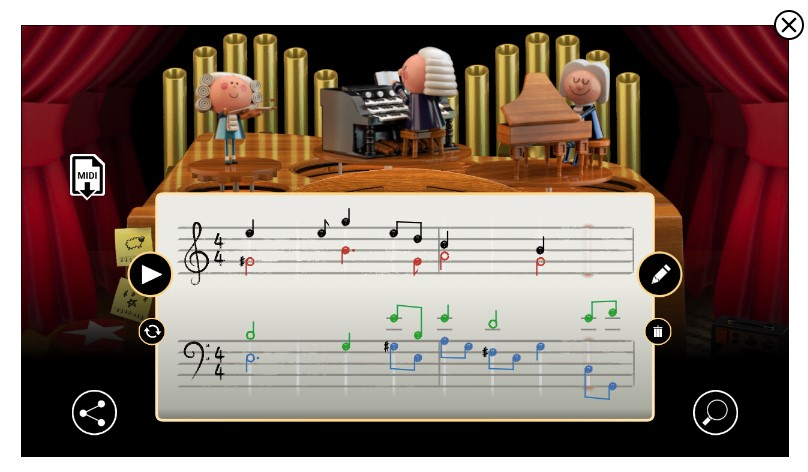
\includegraphics[width=\textwidth]{images/related_works/bachdooldle/bachdoodle.jpg}
    \caption{Bach Doodle application}
    Source: \href{https://www.google.com/doodles/celebrating-johann-sebastian-bach}{BachDoodle}
    \label{fig:bachdoodle}
\end{figure}

% -------------------- Music Representation--------------------

\section{Music Representation}

In this section, I will present different types of inputs the related works use.

\subsection{Audio Signal} 

The first data used to create music is the audio signal. Some works \cite{oord_wavenet:_2016, dieleman_challenge_2018, donahue_adversarial_2019, kalchbrenner_efficient_2018, mehri_samplernn_2017, lu_play_2018} have been done to generate music audio signal.
This signal can be represented either by its waveform \cite{oord_wavenet:_2016}, its Fourier Transform, or its spectrogram (figures \ref{fig:waveform_example}, \ref{fig:spectrogram_example}).

\begin{figure}[H]
   \begin{minipage}{0.5\textwidth}
     \centering
     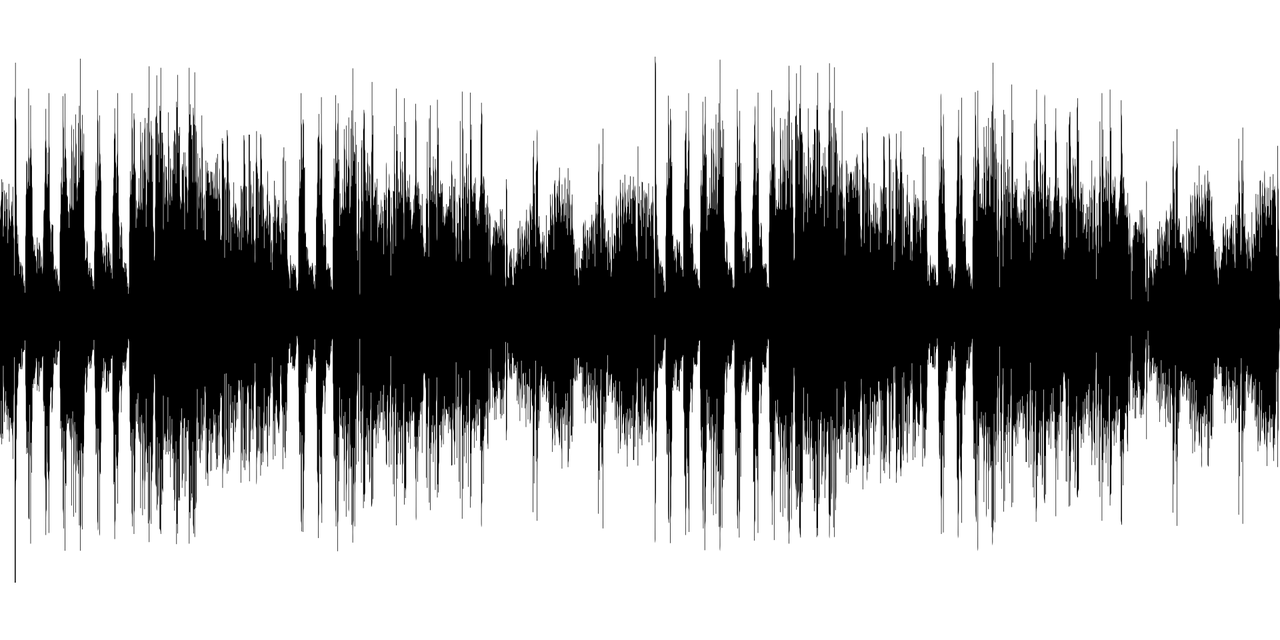
\includegraphics[width=.9\linewidth, height=4cm]{images/music/waveform/waveform.png}
     \caption{Example of an audio waveform}
     Source: \href{https://www.needpix.com/photo/856116/audio-aural-ear-hearing-music-musical-recording-silhouette-sonic}{Needpix.com}
     \label{fig:waveform_example}
   \end{minipage}\hfill
   \begin{minipage}{0.5\textwidth}
     \centering
     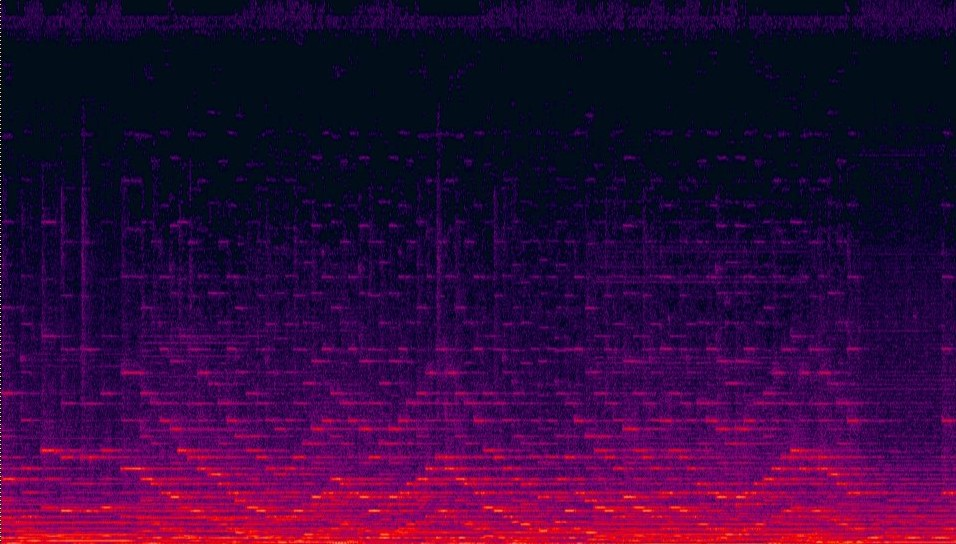
\includegraphics[width=\linewidth, height=4cm]{images/music/spectrogram/spectrogram.jpg}
     \caption{Example of audio spectrogram}
     Source: \href{https://commons.wikimedia.org/wiki/File:Spectrogram_of_Bach\%27s_Chorales_for_Organ.jpg}{Wikipedia}
     \label{fig:spectrogram_example}
   \end{minipage}
\end{figure}

Using the audio signal allows the model to handle every aspects of the song at the same time (instrument, timber, emotion...), and every song in the same way.
The biggest issue of this method is that the number of points need to create a waveform is incredibly huge.
The usual sampling frequency is $48kHz$. 
Therefore, the main difficulty is to stay consistent through time.

\subsection{MIDI Signal}

Most of the works done on music generation use the \textit{MIDI} representation (or any other translation of midi like pianoroll or text). \cite{chuan_modeling_nodate, hadjeres_deepbach:_2016, huang_counterpoint_2017, liang_automatic_2017, adiloglu_machine_2007, herremans_composing_2013, herremans_modeling_2017, boulanger-lewandowski_modeling_2012, lattner_imposing_2018, colombo_learning_2019, brunner_symbolic_2018}

\subsubsection{Pianoroll}

The pianoroll representation can be considered as an image.
Thus, usual deep learning methods on images can  be applied \cite{huang_counterpoint_2017, chuan_modeling_nodate, boulanger-lewandowski_modeling_2012, lattner_imposing_2018, donahue_adversarial_2019}.
The figure \ref{fig:pianoroll_to_array} shows a very naive example of how to convert a pianoroll view to an array.

\begin{figure}[H]
   \begin{minipage}{0.5\textwidth}
     \centering
     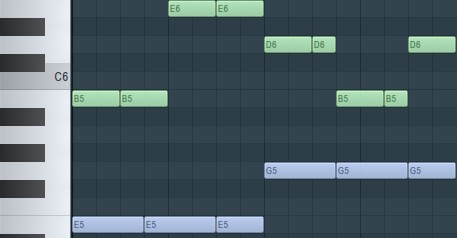
\includegraphics[width=.9\linewidth]{images/music/pianoroll/pianoroll_small.jpg}
   \end{minipage}\hfill
   \begin{minipage}{0.5\textwidth}
     \centering
     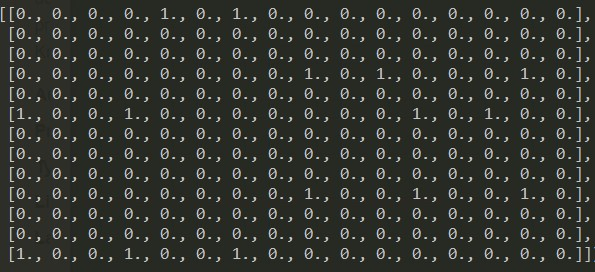
\includegraphics[width=\linewidth]{images/music/pianoroll/pianoroll_small_array.jpg}
   \end{minipage}
 \caption{Example of correspondence between a pianoroll representation and an array}
 \label{fig:pianoroll_to_array}
\end{figure}

\bigskip

Chin-Hua Chuan et al. \cite{chuan_modeling_nodate} introduced another representation to help the model to understand relations between notes.
They use \textit{Tonnetz} matrix \cite{mason_essential_nodate} to represent polyphonic music.
As explained in their paper, \textit{"Tonnetz is a graphical representation used by music theorists and musicologists in order to study tonality and tonal spaces"}.

Instead of encoding notes in a one-dimensional tensor (figure \ref{fig:tonnetz}), they encode them in a 2-dimensional tensor where the relative positions between two notes is meaningful.

The figure \ref{fig:tonnetz} illustrates a common form of tonnetz.
Each node in the tonnetz network represents one of the 12 pitch classes.
The nodes on the same horizontal line follow the circle-of-fifth ordering: the adjacent right neighbor is the perfect-fifth and the adjacent left is the perfect-fourth.
Three nodes connected as a triangle in the network form a triad, and the two triangles connected in the vertical direction by sharing a baseline are the parallel major and minor triads.
For example, the upside-down triangle filled with diagonal lines in the figure \ref{fig:tonnetz} is C major triad, and the solid triangle on the top is C minor triad. Note that the size of the network can be expanded boundlessly; therefore, a pitch class can appear in multiple places throughout the network.

In Chuan's paper, they extended this matrix.
The figure \ref{fig:tonnetz_extended} shows an extended tonnetz matrix example.
They include is this extended matrix the pitch (octave number) which was missing in the first one.

\begin{figure}[h]
    \centering
    \newlength{\MyOtherHeightThree}
    \settoheight{\MyOtherHeightThree}{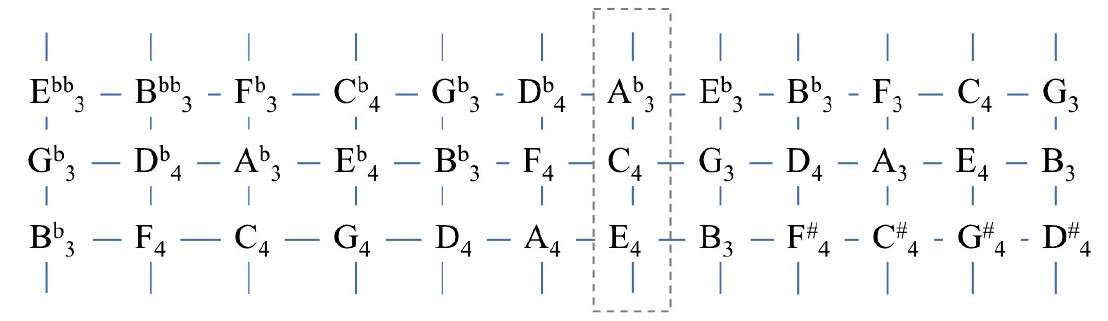
\includegraphics[width=0.9 \textwidth]{images/music/pianoroll/tonnetz_extended.jpg}}
    \begin{subfigure}[t]{0.38\textwidth}
        \centering
        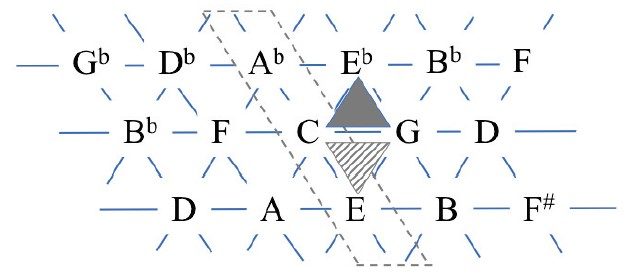
\includegraphics[width=\textwidth]{images/music/pianoroll/tonnetz.jpg}
        \caption{}
        \label{fig:tonnetz}
    \end{subfigure}
    \hfill
    \begin{subfigure}[t]{0.6\textwidth}
        \centering
        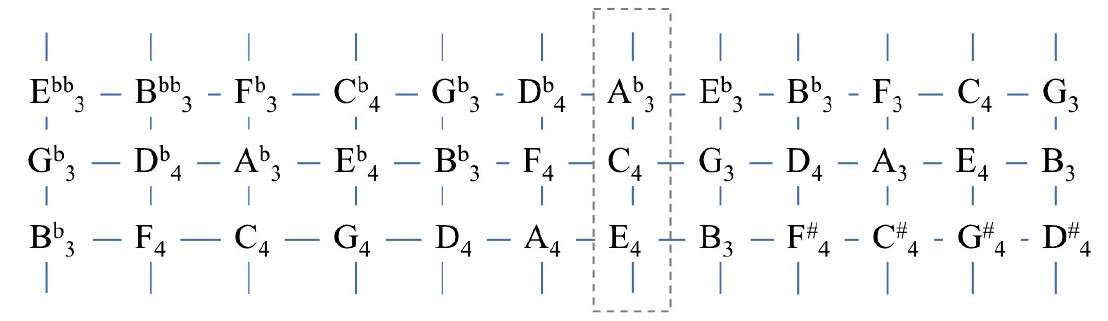
\includegraphics[width=\textwidth]{images/music/pianoroll/tonnetz_extended.jpg}
        \caption{}
        \label{fig:tonnetz_extended}
    \end{subfigure}
    \caption{(a) tonnetz and (b) the extended tonnetz matrix with pitch register}
    Source: Ching-Hua Chuan's paper \cite{chuan_modeling_nodate}.
    \label{fig:tonnetz_representation}
\end{figure}

\subsubsection{Text}

Another approach is to convert the MIDI format into text. \cite{hadjeres_deepbach:_2016}

\begin{figure}[H]
   \begin{minipage}{0.5\textwidth}
     \centering
     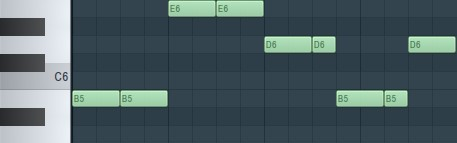
\includegraphics[width=.9\linewidth]{images/music/pianoroll/pianoroll_small_2.jpg}
   \end{minipage}\hfill
   \begin{minipage}{0.5\textwidth}
     \centering
     B5, \_, B5, \_, E6, \_, E6, \_, D6, \_, D6, B5, \_, B5, D6, \_ 
   \end{minipage}
 \caption{Example of correspondence between a pianoroll representation and a text}
 \label{fig:pianoroll_to_text}
\end{figure}

The figure \ref{fig:pianoroll_to_text} shows a simple example of how it is possible to convert an pianoroll view to a text.
However, using text to represent image usually force the framework to work only in a monophonic way.
A common choice of the existing works that working with text is to embed the text into a fix-sized vector using a \texttt{word2vec} \cite{goldberg_word2vec_2014, karani_introduction_2018, rong_word2vec_2016, noauthor_beginners_nodate, mikolov_distributed_2013} model \cite{liang_automatic_2017, herremans_modeling_2017}.

\bigskip

Despite the text constraint, Feynman Liang and al. \cite{liang_automatic_2017} managed to encode polyphonic music in text and use it to correctly train their model: "BachBot".

They quantize time into sixteenth notes (\musEighth). Consecutive frames are separated by a unique delimiter ("\texttt{|||}").
Within each frame, they represent individual notes rather than entire chords.
Each frame consists of four (Soprano, Alto, Tenor, and Bass) \texttt{<Pitch; Tie>} tuples where $\texttt{Pitch} \in \{0; 1; \dots ; 127\}$ represents the MIDI pitch of a note and $\texttt{Tie} \in \{\texttt{True}; \texttt{False}\}$ distinguishes whether a note is tied with a note at the same pitch from the
previous frame or is articulated at the current timestep.
They \textit{order notes within a frame in descending MIDI pitch}.
The figure \ref{fig:relatedwork_bachbot} shows the encoding process.

\begin{figure}[h]
    \centering
    \newlength{\MyOtherHeightTwo}
    \settoheight{\MyOtherHeightTwo}{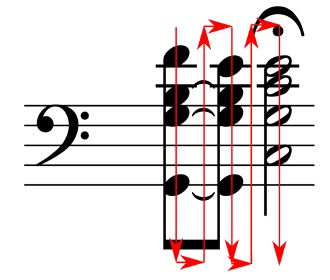
\includegraphics[width=0.9 \textwidth]{images/related_works/bachbot/bachbot_encoding_stave.jpg}}
    \begin{subfigure}[t]{0.28\textwidth}
        \centering
        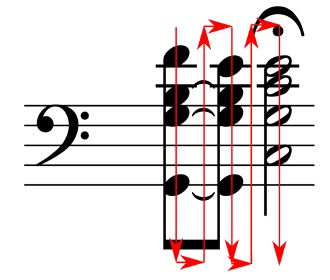
\includegraphics[width=.9 \textwidth]{images/related_works/bachbot/bachbot_encoding_stave.jpg}
        \caption{ {\setstretch{1.}Three musical chords in traditional music notation. The red arrows indicate the order in which notes are sequentially encoded.}}
        \label{fig:relatedwork_bachbot_stave}
    \end{subfigure}
    \hfill
    \begin{subfigure}[t]{0.67\textwidth}
        \centering
        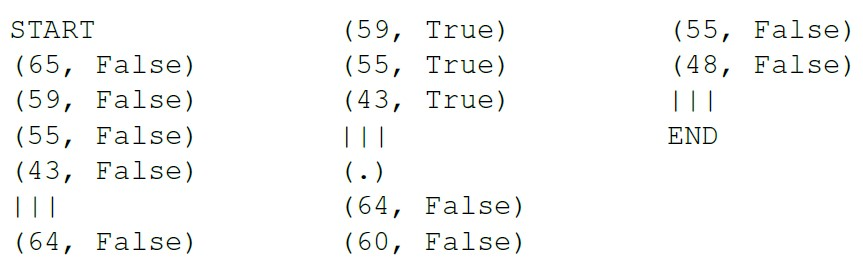
\includegraphics[width=.9 \textwidth]{images/related_works/bachbot/bachbot_encoding_text.jpg}
        \caption{A corresponding sequential encoding of the three chords in an eighth-note time quantization (for illustration, broken over three columns). Each line within a column corresponds to an individual token in the encoded sequence. ||| delimit frames and (.) indicate a fermata is present within the corresponding frame.}
        \label{fig:relatedwork_bachbot_text}
    \end{subfigure}
    \caption{BachBot's example encoding of three musical chords ending with a fermata ("pause") chord}
    Source: Feynman Lian's paper \cite{liang_automatic_2017}.
    \label{fig:relatedwork_bachbot}
\end{figure}


\subsubsection{Chords}

This is the last approach I will describe in this paper.
As the same way as Jazz music, it is possible to simplify the description of a musical piece by writing down the chords.

\begin{figure}[H]
   \begin{minipage}{0.5\textwidth}
     \centering
     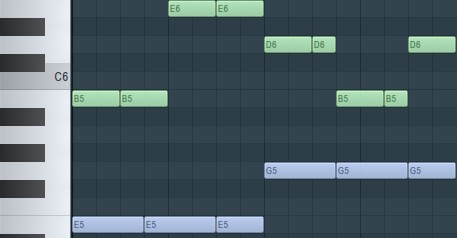
\includegraphics[width=.9\linewidth]{images/music/pianoroll/pianoroll_small.jpg}
   \end{minipage}\hfill
   \begin{minipage}{0.5\textwidth}
     \centering
     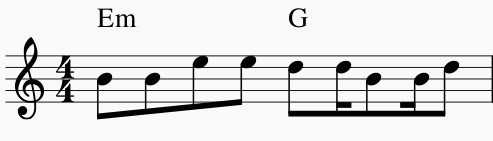
\includegraphics[width=.9\linewidth]{images/music/stave/stave_with_chords.jpg}
   \end{minipage}
 \caption{Example of correspondence between a pianoroll and its chords representation}
 \label{fig:pianoroll_to_chords}
\end{figure}

For instance, in the figure \ref{fig:pianoroll_to_chords}, the bass line can be simplified by considering the chords.
The chords are then writen and be considered as notes.



% TODO: Speak about Chords2Vec
%       Survey descritpion 
% Note that a somehow similar model has been used for polyphonic music generation in
% the BachBot system [66] (analyzed in Section 7.3.1.3). In this model, for each time step, the
% various notes are represented as a sequence and a special delimiter symbol (|||) indicates
% the next time frame (with constant time step of an eighth note (<croche symbol>). Notes are ordered, in a
% descending pitch (soprano voice being the first one). Each note is encoded as its MIDI pitch
% value and a boolean indicating if it is tied to a note at the same pitch from previous frame.
% An example is shown at Figure 4.8, encoding two successive chords (the first having the
% duration of a quarter note) and the second one possessing a fermata (noted as (.)).


% -------------------- Encoding --------------------

\section{Encoding}

\subsection{Features}

It is possible to extract features from the data to help the neural network to understand how music works, like the chords, the current key signature...
\begin{itemize}
    \item The first option is to do it manually and give the features as an input of the model
    \item The second option is to let the model learn it by itself. This is the choice I have made for this project.
\end{itemize}

\subsubsection{Metadata}

The features that can be passed as an input to the model can also be metadata like the time signature or the key of the music...

Deep Bach from Gaëtan Hadjeres et al.'s paper \cite{hadjeres_deepbach:_2016} consider the fermata symbol (figure \ref{fig:fermata}) and the beat subdivision number (an integer between 1 and 4).

\begin{figure}[htbp]
     \centering
     
\includegraphics[width=.1\linewidth]{images/music/symbols/fermata.png}
     \caption{Fermata symbol}
     Source: \href{https://publicdomainvectors.org/en/free-clipart/Music-symbol/70183.html}{publicdomainvector}
     \label{fig:fermata}
\end{figure}

In this project I chose to not include any metadata in the model because of the difficulty to find or reconstruct them for the available dataset.
However, I not intentionally gives to the model the information about the beats number and subdivisions by considering the entire measure as one input.

\bigskip

Another way to help the model by giving it information without actually passing metadata is to normalize the data.
For example, BachBot \cite{liang_automatic_2017} and other works \cite{chuan_modeling_nodate, boulanger-lewandowski_modeling_2012} transpose all their dataset in either C major or A major key.

For the same reason as not passing metadata, I don't normalize the data before training my models.

% TODO say I put everything in C major or A minor

\subsection{Tensor encoding}

It is possible to extract two different methods on how to encode the tensor which will be given to the neural network

The first method is the \textit{value encoding}.
It means that the values in the input and/or output tensor are actually meaningful.
For example, it can be an integer which is the pitch of a note.

The second method is called \textit{item encoding}.
Instead of having the number of the pitch in the tensor (let's say $60$), it will be a very sparse tensor with a bunch on $0$ and a $1$ at the position $60$ in the pitch dimension.
This values stored in the tensors can be considered as \textit{activation} values.
This is the retained method in my Dissertation.


\section{Architectures}


In this section, I will present different architectures that have already been used for music generation. It will expose the architecture of my project in the section \ref{sec:rmvae}.


\subsection{RBM}

The RBM architecture is explained in the section \ref{sec:back:rbm}.

Nicolas Boulanger-Lewandowski et al. \cite{boulanger-lewandowski_modeling_2012} use an RBM based model RTRBM \cite{sutskever_recurrent_nodate, mittelman_structured_nodate} and created their own architecture called RNN-RBM.
They applied their model on different MIDI dataset to create polyphonic music.

Stefan Lattner et al. \cite{lattner_imposing_2018} use another RBM based model called C-RBM \cite{norouzi_convolutional_nodate, norouzi_stacks_nodate}.
They apply this model on pianoroll images.
They also implement a different constraints like their self-similarity constraint to specify a repetition structure (e.g. AABA) in the general music piece.


\subsection{NADE}
\label{sec:rw:nade}

The NADE architecture is explained in the section \ref{sec:back:nade}.

And as an example, Cheng-Zhi Anna Huang et al. \cite{huang_counterpoint_2017} use an orderless NADE \cite{uria_deep_2014} to generate music. They introduce COCONET, a deep convolutional model to reconstruct partial scores.
It consists of a corruption process that masks out a subset $x_{\neg C}$ of variables, followed by a process that independently resamples variables $x_{i}$ (with $i \not \in C$) according to the distribution $p_{\theta} (x_i | x_C )$ emitted by the model with parameters $\theta$.


The figure \ref{fig:coconet_process} illustrates how the process works.
At each step, a random subset of notes is removed, and the model is asked to infer their values.
New values are sampled from the probability distribution put out by the model, and the process is repeated.

Google also Bach Doodle \cite{huang_bach_2019}, an online tool re-implementing COCONET in Tensorflow.js \cite{noauthor_tensorflowjs_nodate} which harmonizes a melody given by the user.


\subsection{AE}

The AutoEncoder architecture is explained in the section \ref{sec:back:ae}.

This is the most common architecture used for music generation at the time I am writing this report.
The AutoEncoder can be recurrent  \cite{liang_automatic_2017, chuan_modeling_nodate, hadjeres_deepbach:_2016, kalchbrenner_efficient_2018, mehri_samplernn_2017} as Feynman Liang et al.'s BachBot \cite{liang_automatic_2017} or not \cite{dieleman_challenge_2018}.

For instance, BachBot \cite{liang_automatic_2017} and DeepBach \cite{hadjeres_deepbach:_2016} use an encoder/decoder architecture with LSMT layers on the latent space. \cite{chuan_modeling_nodate}

Soroush Mehri et al. \cite{mehri_samplernn_2017} or Nal Kalchbrenner et al. \cite{kalchbrenner_efficient_2018} have created different AE architecture to synthesize audio waveform and can be applied to music sounds.

\subsection{VAE}

The Variational AutoEncoder architecture is explained in the section \ref{sec:back:vae}. 

Sander Dieleman et al. \cite{dieleman_challenge_2018} use a VAE (or more precisly a VQ-VAE \cite{van_den_oord_neural_2017}  or a AMAE \cite{dieleman_challenge_2018}) to encode audio waveform and reconstruct it with a stylistic consistency accross tens of seconds.


\subsection{RMVAE}

Since I created this new architecture, there is no existing work using this architecture.
My project is, for now, the only work done using a Recurrent Multimodal Variational AutoEncoder to generate music.

The RMVAE's architecture is explained in the section \ref{sec:rmvae}

\subsection{GAN}

The Generative Adversarial Network Architecture is explained in the section \ref{sec:back:gan}

For instance, the model WaveGan from Chris Donahue et al. \cite{donahue_adversarial_2019} use a GAN architecture to synthesize audio waveform in several domains including drums and piano.

Gino Brunner et al. \cite{brunner_symbolic_2018} use CycleGAN \cite{zhu_unpaired_2018} to create a model able to apply a style transfer on musical pieces (between jazz, pop and classical style).

\subsection{Reinforcement learning}

% TODO : Speek about reinforcement learning

\section{Generation Process}

In this section, I will enumerate different techniques to generate music from different model architectures.

\subsection{Sampling}

The sampling process can either be done with a VAE, or an GAN architecture \cite{donahue_adversarial_2019}.

A VAE keeps its latent space distribution as the standard normal distribution $\mathcal{N}(0, 1)$.
Thus, by giving a random vector sampled from a standard normal distribution $\mathcal{N}(0, 1)$, the decoder will construct an output similar to the dataset the model trained on.

The generator of a GAN has been trained to generated consistent data from noise.
Then, the process generation for a GAN is to give a random input from a standard normal distribution to generator.

\subsection{Input Manipulation}

Generating music by manipulating the input is typically how style transfer algorithms work \cite{shetty_neural_2019, gatys_neural_2015, li_universal_2017}.
The input is considered as a variable which is updated to minimize a loss function constructed from a content target and a style target.
The content similarities between the input and the content target is reduced through the iterations.
In the same way, the style similarities between the style target and the input will minimized.

This process works well for images to create a new image combining content and style from 2 different images.
People tried to apply the same methods on music \cite{kaliakatsos-papakostas_conceptual_2017, hung_musical_2019, brunner_symbolic_2018, lu_play_2018}, but as Shuqi et al. \cite{dai_music_2018} say, music is more complex and has several level of style (timber, performance and composition).
Therefor, creating a music style transfer algorithm is more complicated than for images and the results are currently not as good.

\subsection{Feed forward and RNN architecture}

This is the easiest and most common generation process through all the works \cite{liang_automatic_2017, chuan_modeling_nodate, huang_counterpoint_2017}, and this is the one I chose for this project.
And input is given to the model.
The model returns an output.
The figure \ref{fig:feed_forward_generation_process} illustrates this process.
This output can be the next frame/beat/measure (in my case, a measure) of the music.

I also chose this generation process for my project.
In my case, the model returns the next measure of the music.

\begin{figure}[h]
\begin{center}
    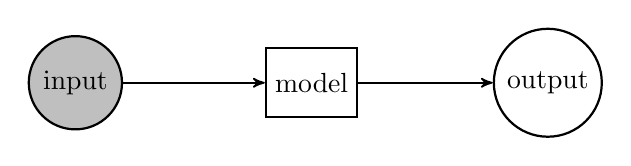
\begin{tikzpicture}[->, >=stealth', auto, semithick, node distance=3cm]
    \tikzstyle{every state}=[fill=white,draw=black,thick,text=black,scale=1]
    \node[state, rectangle](model){model};
    \node[state, fill=lightgray](input)[left of=model]{input};
    \node[state](output)[right of=model]{output};
    \path
        (input) edge    node{}  (model)
        (model) edge    node{}  (output);
    \end{tikzpicture}
\caption{Feed forward generation process}
\label{fig:feed_forward_generation_process}
\end{center}
\end{figure}

\subsubsection{DeepBach}

To give an illustration, DeepBach \cite{hadjeres_deepbach:_2016} uses a Markov Chain Monte Carlo algorithm to re-harmonize a song and transform it. 
From the existing song, it re-predicting every notes one by one.
The algorithm is describe in the figure 

\begin{figure}[htbp]
     \centering
     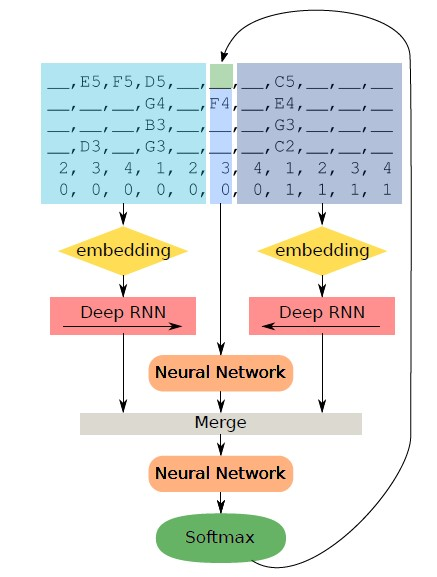
\includegraphics[width=.5\linewidth]{images/related_works/deepbach/deepbach_algo.jpg}
     \caption{Graphical representation of DeepBach's neural network architecture for the soprano prediction}
     Source: DeepBach paper \cite{hadjeres_deepbach:_2016}
     \label{fig:relatedworks:deepbach_architecture}
\end{figure}

% ----------------------------------------------------------------------------------------------------
% Contribution
% ----------------------------------------------------------------------------------------------------
\newpage
\chapter{Contribution}
\label{chap:contribution}

% -------------------- Objectives --------------------

\section{Objectives}
\label{sec:objectives}

As a musician, I wanted to create an model architecture who could copy the way I think about music.
The challenge is to use only one trained model to be able to 
\begin{itemize}
    \item Generate music with several musical parts (meaning several instruments)
    \item Create a accompaniment from a melody
    \item Create a melody from a accompaniment
    \item Create a musical part from other musical parts
\end{itemize}
The created model can also handle missing data (for example a missing measure from a instrument).

To summarize, the objective is to create a unique trained model which can generate or arrange a musical piece whatever is already present or missing.

\section{Data representation}
\label{sec:data_represetation}

This project works with MIDI data. These music representation is explained in the section \ref{sec:midi}. \\
The shortest beat division is a quarter of a beat (sixteenth note: \musSixteenth) \\
The considered music are binary and with 4 beats per measure. \\
Because I think that a measure can be consider as an entire object (with its rhythm, its chords ...), I chose to divide music by measure. Thus, a time step for the neural network is the representation of an entire measure.
The shape of shape of a tensor representing a measure will be \texttt{(16, 128, channels)}:
\begin{itemize}
    \item \texttt{16} is the number of sixteenth notes (\musSixteenth) is a measure.
    \item \texttt{128} is the number of different MIDI notes possible (from $0$ to $127$).
    \item \texttt{channels} $\in \{1, 2\}$ is explained in the sections \ref{sec:poly} and \ref{sec:mono}.
\end{itemize}

The number of instruments is fixed and are different inputs of the neural network.
Hence, for one instrument, its associated tensor has a shape of \texttt{(nb\_measures, 16, 128, channels)}. \texttt{nb\_measures} is the number of measures considered.

\subsection{Polyphonic music}
\label{sec:poly}

For polyphonic music, the number of \texttt{channels} it $2$.

The first channel is called the \textit{activation} channel. The value is either $1$ for a played note or $0$ for a non-played note.

The second channel is called the \textit{duration} channel. The value is an integer corresponding of \textit{"how many sixteenth notes (\musSixteenth) it lasts"}.
The table \ref{tab:duration} shows the correspondence between the value of the duration channel and the musical length representation.

\begin{table} [ht]
    \begin{center}
        \begin{tabular} {c|c}
            Duration value & Musical length \\
            \hline
            $1$ & \musSixteenth \\
            $2$ & \musEighth \\
            $3$ & \musEighthDotted \\
            $4$ & \musQuarter \\
            $5$ & $\musQuarter_{\smile}$\musSixteenth \\
            $6$ & \musQuarterDotted \\
            $7$ & $\musQuarter_{\smile} \musEighthDotted$ \\
            $8$ & \musHalf \\
            $9$ & $\musHalf_{\smile} \musSixteenth$ \\
            $10$ & $\musHalf_{\smile} \musEighth$ \\
            $11$ & $\musHalf_{\smile} \musEighthDotted$ \\
            $12$ & \musHalfDotted \\
            $13$ & $\musHalfDotted_{\smile} \musSixteenth$ \\
            $14$ & $\musHalfDotted_{\smile} \musEighth$ \\
            $15$ & $\musHalfDotted_{\smile} \musEighthDotted$ \\
            $16$ & \musWhole \\
        \end{tabular}
        \caption{Correspondence between duration value and musical length}
        \label{tab:duration}
    \end{center}
\end{table}

If a note is note activated (activation channel $ = 0$), then the duration channel is set to $0$ too.

\begin{equation}
    \texttt{channel}_{\texttt{activation}} = 0 \iff \texttt{channel}_{\texttt{duration}} = 0
\end{equation}

\subsection{Monophonic Music}
\label{sec:mono}

The goal was too reduce the memory space a simplify the model for monophonic music.
Since monophonic music can means there is a maximum of one note played simultaneously at a time $t$, I chose to not consider the rests and consider that every notes last until an another note is played.\\
Thus, I get read of duration channel and the number of \texttt{channels} $ = 1$.

An \textit{additional note} is inserted which is the $note_{continue}$.
The tensor shape of a step is now \texttt{(16, 128 + 1, 1)}.
When $note_{continue}$ is set to $1$, it means there is no new note to be played.
And when $note_{continue}$ is set to $0$, it means a new notes has to be played.

\begin{equation}
    note_{continue} = 1 \implies \forall~ note \in notes_{[0:128]}, note = 0
\end{equation}

\begin{equation}
    note_{continue} = 0 \implies \exists!~ note \in notes_{[0:128]}, note = 1
\end{equation}

And since I consider in this part only monophonic music, there is only on note (included $note_{continue}$ per each time division)

\begin{equation}
    \exists! note \in notes_{[0:129]}, note = 1
\end{equation}

% -------------------- Architecture --------------------

\section{RMVAE Architecture}
\label{sec:rmvae}

I have created a new architecture which is able to handle all the objectives defined in the section \ref{sec:objectives}.

To do so, I continued the work of Mike We et al. \cite{wu_multimodal_2018} and their Multimodal Varational AutoEncoder (MVAE) (see section \ref{sec:back:mvae}) and I simplified the work of Tan Zhi-Xuan et al. \cite{tan_factorized_2019} and their Multimodal Deep Markov Models (MDMM) (see section \ref{sec:back:mdmm}).

\subsection{Global Architecture}

I use the capability of the MVAE to reconstruct data and handle several modalities at the same time with the help of the product of expert operation.
But because the MVAE doesn't handle time across the data, it had to be transformed.
And that is basically what does the MDMM.
However, the training process of a MDMM is quite complicated and slow. Because of this reason, I came up with a novel architecture that I call RMVAE (Recurrent Multimodal Varational AutoEncoder). This architecture is describe in the figure \ref{fig:rmvae_architecture}.


% Good example how to use tikz:
% https://tex.stackexchange.com/questions/193694/drawing-graph-of-markov-chain-with-patches-using-tikz
\begin{figure}
\begin{center}
    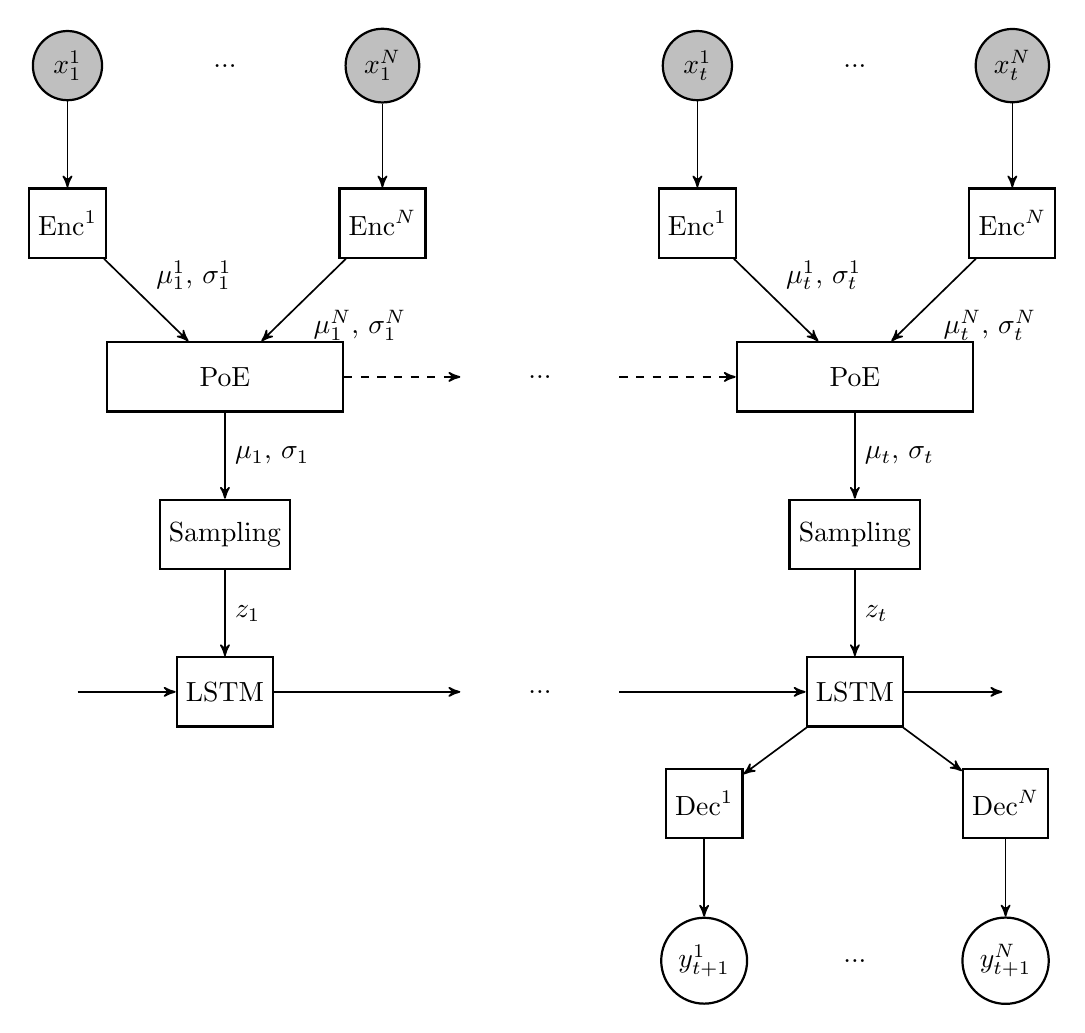
\begin{tikzpicture}[->, >=stealth', auto, semithick, node distance=2cm]
    \tikzstyle{every state}=[fill=white,draw=black,thick,text=black,scale=1]
    \node[state, fill=lightgray](x11)[]{$x_1^1$};
    \node[](dots1)[right of=x11]{$...$};
    \node[state, fill=lightgray](x1n)[right of=dots1]{$x_1^N$};
    \node[state, rectangle](enc11)[below of=x11]{$\text{Enc}^1$};
    \node[state, rectangle](enc1n)[below of=x1n]{$\text{Enc}^N$};
    \node[state, rectangle, below=1.5cm, minimum width=3cm](poe1) at ($(enc11)!0.5!(enc1n)$) {PoE};
    \node[state, rectangle](samp1)[below of=poe1]{Sampling};
    \node[state, rectangle](lstm1)[below of=samp1]{LSTM};
    
    \node[state, fill=lightgray, right=2cm](xt1)[right of=x1n]{$x_t^1$};
    \node[](dots2)[right of=xt1]{$...$};
    \node[state, fill=lightgray](xtn)[right of=dots2]{$x_t^N$};
    \node[state, rectangle](enct1)[below of=xt1]{$\text{Enc}^1$};
    \node[state, rectangle](enctn)[below of=xtn]{$\text{Enc}^N$};
    \node[state, rectangle, below=1.5cm, minimum width=3cm](poet) at ($(enct1)!0.5!(enctn)$) {PoE};
    \node[state, rectangle](sampt)[below of=poet]{Sampling};
    \node[state, rectangle](lstmt)[below of=sampt]{LSTM};
    
    \node[minimum width=2cm](lstmdots) at ($(lstm1)!0.5!(lstmt)$) {...};
    
    \node[](lstm0)[left of=lstm1]{};
    \node[](lstminf)[right of=lstmt]{};
    
    \node[](dec1)[below of=lstm1]{};
    \node[state, rectangle, left=0.5cm](dect1)[below left of=lstmt]{$\text{Dec}^1$};
    \node[state, rectangle, right=0.5cm](dectn)[below right of=lstmt]{$\text{Dec}^N$};
    \node[state](yt1)[below of=dect1]{$y_{t+1}^1$};
    \node[state](ytn)[below of=dectn]{$y_{t+1}^N$};
    \node[](dots3) at ($(yt1)!0.5!(ytn)$)   {...};
    
    \node[minimum width=2cm](dotspoe) at ($(poe1)!0.5!(poet)$) {...};
    
    \path
        (x11)   edge    node{}      (enc11)
        (x1n)   edge    node{}      (enc1n)
        (enc11) edge    node{$\mu_1^1$, $\sigma_1^1$}   (poe1)
        (enc1n) edge    node{$\mu_1^N$, $\sigma_1^N$}   (poe1)
        (poe1)  edge    node{$\mu_1$, $\sigma_1$}   (samp1)
                edge[dashed]    node{} (dotspoe)
        (dotspoe)   edge[dashed]    node{}  (poet)
        (samp1) edge    node{$z_1$}   (lstm1)
        
        (xt1)   edge    node{}      (enct1)
        (xtn)   edge    node{}      (enctn)
        (enct1) edge    node{$\mu_t^1$, $\sigma_t^1$}   (poet)
        (enctn) edge    node{$\mu_t^N$, $\sigma_t^N$}   (poet)
        (poet)  edge    node{$\mu_t$, $\sigma_t$}   (sampt)
        (sampt) edge    node{$z_t$}   (lstmt)
        
        (lstm0) edge    node{}  (lstm1)
        (lstm1) edge    node{}  (lstmdots)
        %        edge    node{}  (dec1)
        (lstmdots)  edge    node{}  (lstmt)
        (lstmt) edge    node{}  (lstminf)
                edge    node{}  (dect1)
                edge    node{}  (dectn)
        (dect1) edge    node{}  (yt1)
        (dectn) edge    node{}  (ytn);
        
    \end{tikzpicture}
\caption{Architecture of the RMVAE}
\label{fig:rmvae_architecture}
\end{center}
\end{figure}

\subsection{Encoder}

Each instruments (each modalities) has its own encoder.
As explained in the section \ref{sec:data_represetation}, the input tensor for one instrument has the following shape: \texttt{(nb\_steps, 16, 128, channels)}.
For a given instrument $i$, and a given step $t$, the tensor (with a shape of \texttt{(16, 128, channels)}) can be considered as a pianoroll image, hence usual imaging operations can be applied.

The encoder $\text{Enc}^i$ process each steps of a the instrument $i$. And encoder is composed of:
\begin{enumerate}
    \item Convolutional layers and pooling layers
    \item Fully Connected layers
\end{enumerate}
The general architecture of the encoder is showed in the figure \ref{fig:rmvae_encoder}.

\begin{figure}[h]
    \centering
    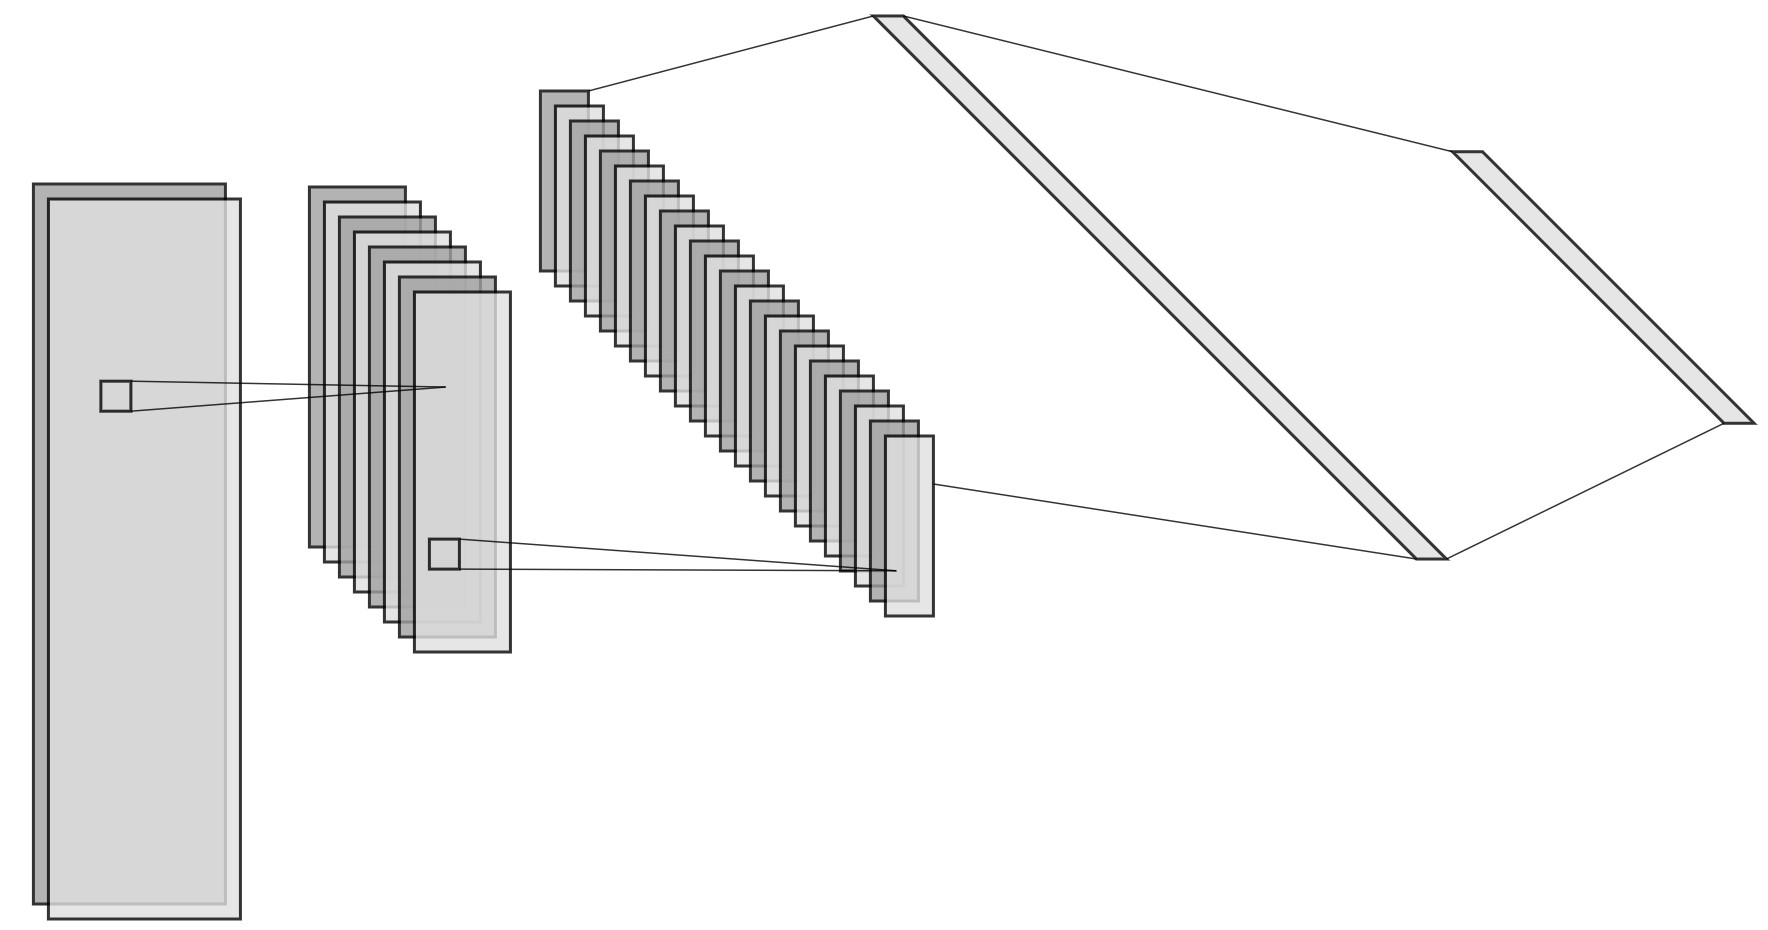
\includegraphics[width=0.8\textwidth]{images/nn/architectures/rmvae/encoder.jpg}
    \caption{RMVAE encoder architecture}
    \label{fig:rmvae_encoder}
\end{figure}

The filter sizes of the convolutional layers are \texttt{(5, 5)}.
I chose this dimension so the receptive field of the first layer is a third major interval and an entire beat.

\subsection{PoE}

For a given instrument $i$ and a given step $t$, the output of the encoder $\text{Enc}^i$ will then go through 2 different FC layers $\text{fc}^i_\mu$ and $\text{fc}^i_\sigma$ which will return the mean and variance of the encoded normal distribution (figure \ref{fig:rmvae_poe_fc}).

\begin{figure}[h]
    \centering
    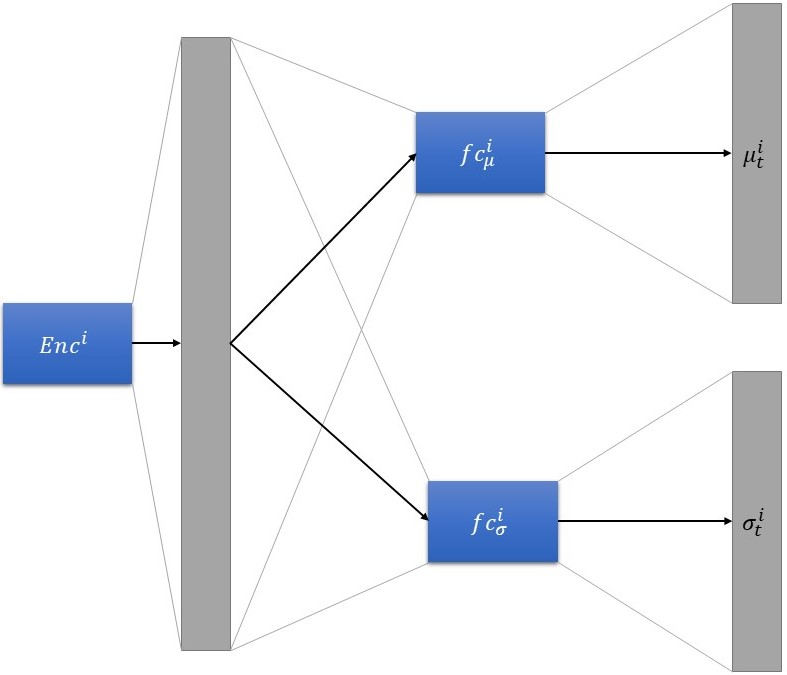
\includegraphics[width=0.6\textwidth]{images/nn/architectures/rmvae/poe_fc.jpg}
    \caption{RMVAE PoE Fully Connected layers}
    \label{fig:rmvae_poe_fc}
\end{figure}

Then, for a given step $t$, all the distribution representation go through the PoE layer to be combined and sampled as shown in the figure \ref{fig:mvae_architecture}.

\subsection{Recurrent layers}

I have now all the latent represenations for every steps : $\{z_1, ..., z_T\}$.

\subsubsection{LSTM cells}

To learn, how this latent space evolves through time, RMVAE uses recurrent layers with LSTM cells (figures \ref{fig:rnn} , \ref{fig:lstm}).
This is shown in the figure \ref{fig:rmvae_lstm}.


\begin{figure}
\begin{center}
    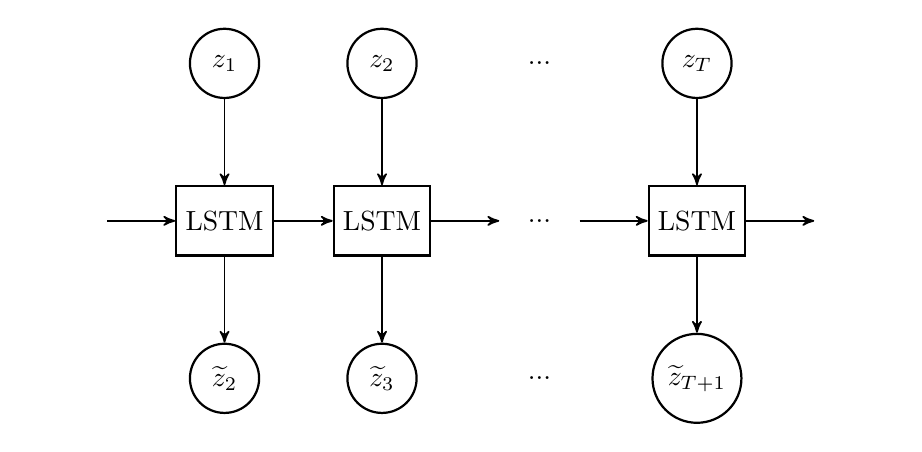
\begin{tikzpicture}[->, >=stealth', auto, semithick, node distance=2cm]
    \tikzstyle{every state}=[fill=white,draw=black,thick,text=black,scale=1]
    \node[state](z1)[]{$z_1$};
    \node[state](z2)[right of=z1]{$z_2$};
    \node[](dotsz)[right of=z2]{...};
    \node[state](zt)[right of=dotsz]{$z_T$};
    
    \node[state, rectangle](lstm1)[below of=z1]{$\text{LSTM}$};
    \node[state, rectangle](lstm2)[below of=z2]{$\text{LSTM}$};
    \node[minimum width=1cm](dotslstm)[below of=dotsz]{...};
    \node[state, rectangle](lstmt)[below
    of=zt]{$\text{LSTM}$};
    
    \node[state](zp2)[below of=lstm1]{$\widetilde{z}_2$};
    \node[state](zp3)[below of=lstm2]{$\widetilde{z}_3$};
    \node[](dotsz)[below of=dotslstm]{...};
    \node[state](zpt1)[below of=lstmt]{$\widetilde{z}_{T+1}$};
    
    \node[minimum width=1cm](whitelstmleft)[left of=lstm1]{};
    \node[minimum width=1cm](whitelstmright)[right of=lstmt]{};
    
    % -----
    
    \draw (z1) -> (lstm1);
    \draw (z2) -> (lstm2);
    \draw (zt) -> (lstmt);
    
    \draw (whitelstmleft) -> (lstm1);
    \draw (lstm1) -> (lstm2);
    \draw (lstm2) -> (dotslstm);
    \draw (dotslstm) -> (lstmt);
    \draw (lstmt) -> (whitelstmright);
    
    \draw (lstm1) -> (zp2);
    \draw (lstm2) -> (zp3);
    \draw (lstmt) -> (zpt1);
    
    \end{tikzpicture}
\end{center}
\caption{RMVAE LSTM layer}
\label{fig:rmvae_lstm}
\end{figure}

\subsubsection{RPoE}
\label{sec:rpoe}

To try to catch the time dependency as good as possible, I implemented a new layer architecture. I call it Recurrent Product of Experts (RPoE).

The result of the Product of Experts at the step $t$ is given as a modality for the Product of Experts at the step $t+1$.

The architecture is displayed in the figure \ref{fig:rpoe_architecture}.

\begin{figure}[h]
    \centering
    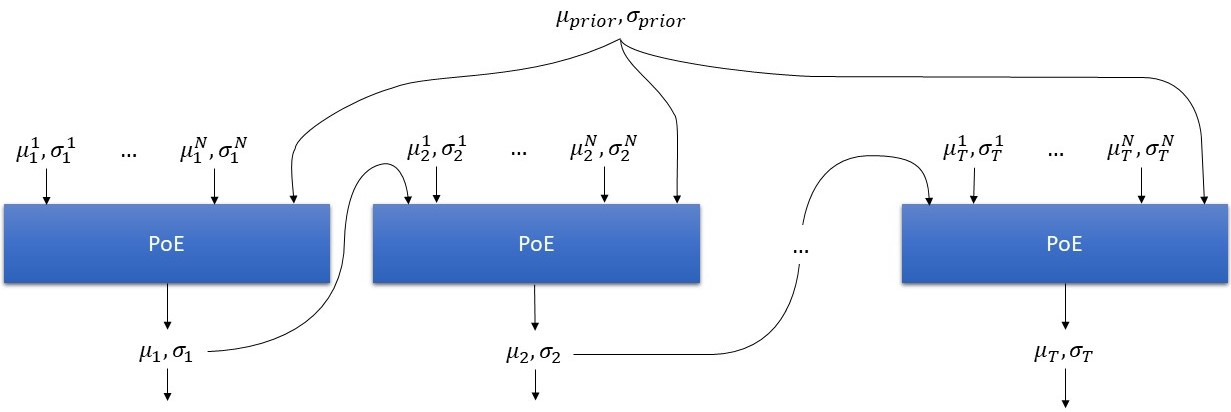
\includegraphics[width=\textwidth]{images/nn/architectures/rmvae/rpoe_architecture.jpg}
    \caption{RPoE architecture}
    \label{fig:rpoe_architecture}
\end{figure}


\subsection{Decoder}

Each instruments (each modalities) has its own decoder.
The decoder $\text{Dec}^i$ associated to the instrument $i$ will, for a given step $t$, reconstruct back the output with the same shape as the input (\texttt{(16, 128, channels)}).

A decoder is composed of:
\begin{enumerate}
    \item Fully Connected layers
    \item Transposed Convolutional layers
\end{enumerate}
The dimensions of the layers of the encoder $\text{Enc}^i$ are the same as the dimensions of the decoder $\text{Dec}^i$.

The decoder global architecture is showed in the figure \ref{fig:rmvae_decoder}.

\begin{figure}[ht]
    \centering
    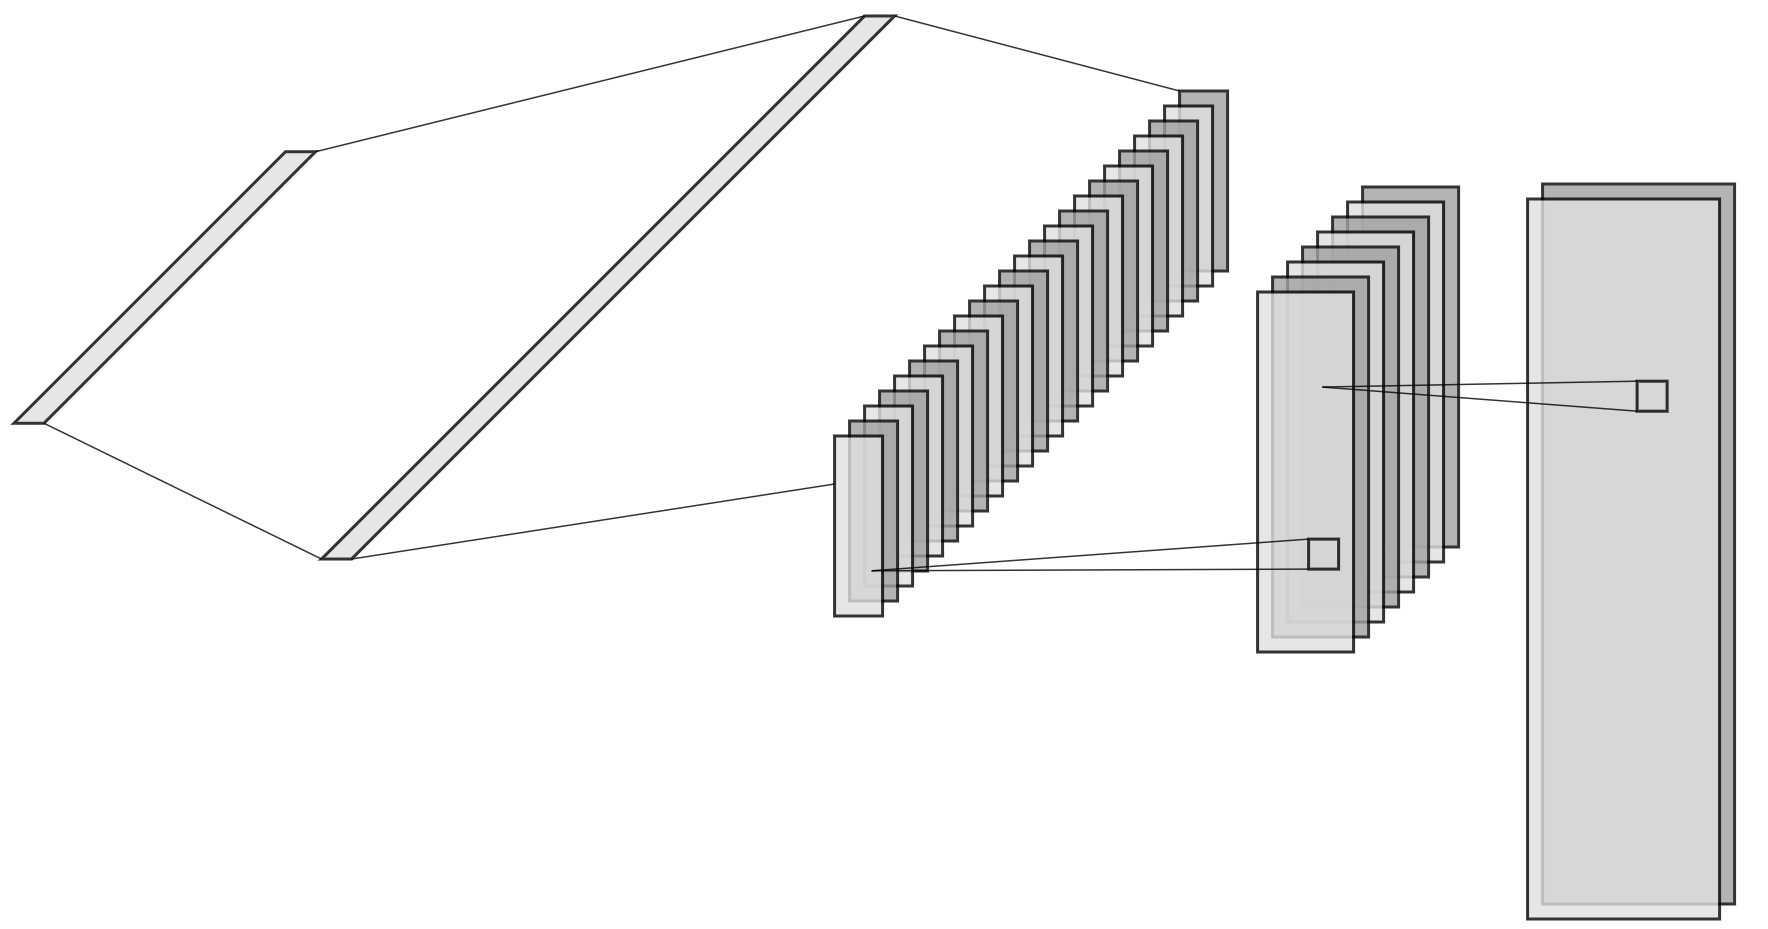
\includegraphics[width=\textwidth]{images/nn/architectures/rmvae/decoder.jpg}
    \caption{RMVAE decoder architecture}
    \label{fig:rmvae_decoder}
\end{figure}

\subsection{Last layer}

The last layer of the NN is a Fully Connected layer with a well chosen activation function.

\subsubsection{Polyphonic Music}

For polyphonic music (section \ref{sec:poly}), the activation function is a \textit{sigmoid} function for the \texttt{channel 1} which represents the activation of the notes.
The activation function for the \texttt{channel 2} is a \textit{ReLU} function.

\subsubsection{Monophonic Music}

For monophonic music (section \ref{sec:mono}), the activation function is s \textit{sigmoid} function for the \textit{additional note} (index 128: $note_{continue}$) because it is an activation note indicating if it wants to continue the previous note or play a new one. And for the other 128 notes, the activation function is a \textit{softmax} function since only one note can be played at the same time.

At the beginning of my project, I was considering the $note_{continue}$ as a \textit{normal note} and simply apply a softmax across all the notes.
But the result was disappointing: the frequency of $note_{continue}$ in the dataset was to high.
The network wasn't generating anything because the $note_{continue}$ had the highest probability.

% -------------------- Loss Function --------------------

\section{Loss Function}
\label{sec:loss}

For this project, I created new loss functions to help the network to understand how music works.
As a musician, I asked myself how I would proceed if I was given the same task as the NN (generation of music, accompaniment...).
This is how I got the idea to create those new loss functions.

In a song, when a musician is playing, it is not possible for him play every one of the 12 notes whenever he wants.
A music usually follows a pattern, a chord progression, and he has to follows it.
From the chords played, the scale, some notes will sounds better to the human ears than other.
But there is no \textit{"ground truth"} for a solo part for example.
Every solo can be considered as a \textit{"ground truth"} if it sounds nice.
And I wanted my model to be able to \textit{improvise}, generate new music.

I got the idea of helping the model to do \textit{acceptable mistakes} and restraint it do \textit{unacceptable mistakes}.
In other word, during the training part, it the model doesn't hit the note it should have hit, I don't want to \textit{punish} it to much with a high loss value if the note sounds actually nice with the music.
On the other side, I want to \textit{punish} it if the note it hits is completely wrong with a higher loss value.

To summarize what I previously just said, during the training part, if the model hits a note which sounds nice, a reward is given by adding a negative number to the loss.
If the hit note doesn't sound nice, then a penalty is given by adding a positive number to the loss.
The algorithm \ref{alg:loss} describe the process.

\begin{algorithm}
    \begin{algorithmic}[1]
        \Require{$noteTruth, notePredict$}
        \Ensure{$loss$}
        \Statex
        \State {$reward > 0, penalty >0$}
        \Function{Loss}{$noteTruth, notePredict$}
            \State {$loss \gets \texttt{commonLoss}(noteTruth, notePredict)$}
            \If{$\texttt{soundsGood}(notePredict)$}
                \State $loss \gets loss - reward$
            \Else
                \State $loss \gets loss + penalty$
            \EndIf
            \State \Return {$loss$}
        \EndFunction
    \end{algorithmic}
    \caption{Add a Reward or a penalty to the generated note}
    \label{alg:loss}
\end{algorithm}

The difficulty is to create the function \texttt{soundsGood} from the algorithm \ref{alg:loss}.
The following sections describe the idea I have had to know whether a note sounds nice or not.

\subsection{Scale}

I call this loss function \textit{Scale} because the idea is to reconstruct the \textit{local scale}.
This loss function takes as inputs all the instruments output:
\begin{center}
$\texttt{Scale}(truth, predict)$
\end{center}
where the shape of the input tensors is \texttt{(nb\_instruments, 16, 128)} for both which the represent the activated notes (where there is a 1) of every instruments for the next measure. The figure \ref{fig:loss_scale} shows the operations of this function.

The idea is to take all the played notes for all the instruments in the truth tensor.
Because the same note from different octaves should be considered as the same note, I apply a segment sum to get in the end a tensor of shape \texttt{(12,)} which corresponds to the 12 notes.
The details of the segment sum operation are explained in the appendix \ref{appendix:segment_sum}.


\begin{figure}[h]
\begin{center}
    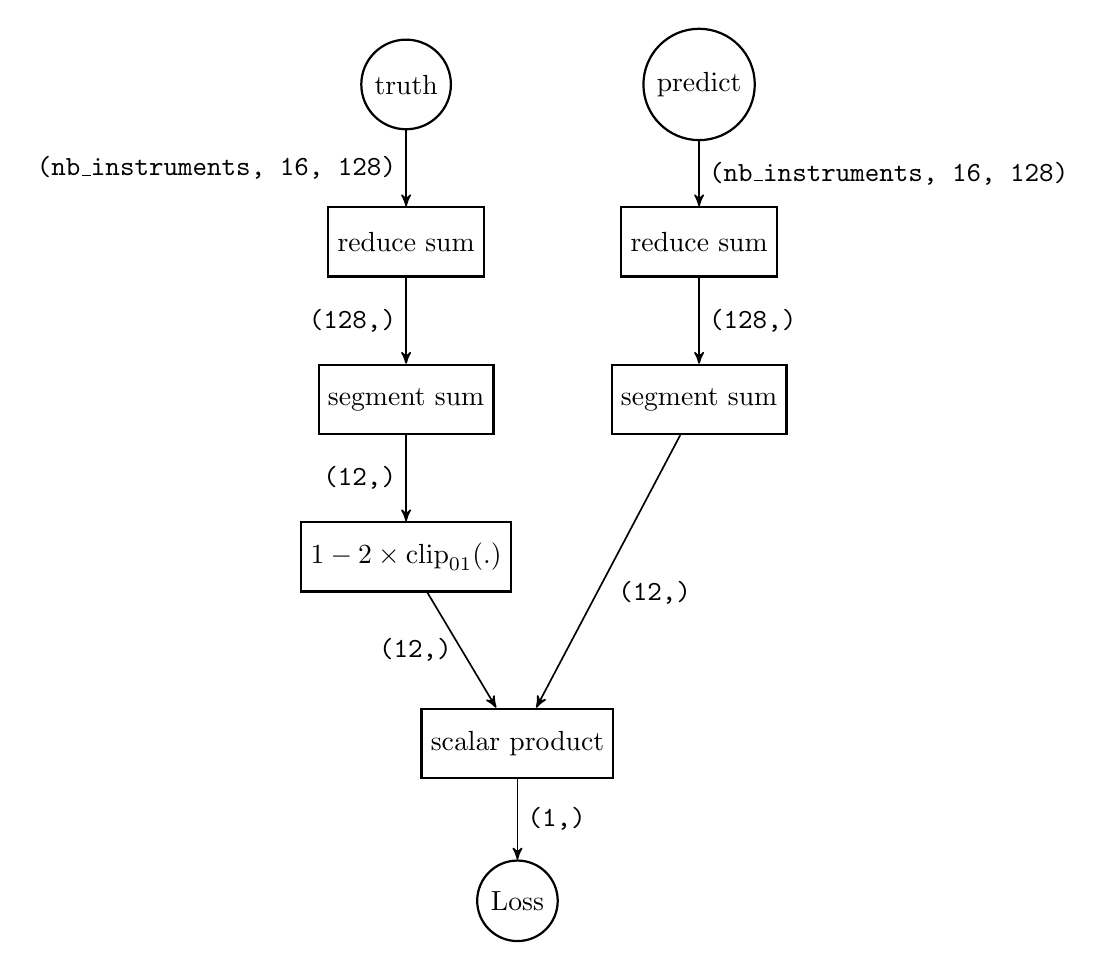
\begin{tikzpicture}[->, >=stealth', auto, semithick, node distance=2cm]
    \tikzstyle{every state}=[fill=white,draw=black,thick,text=black,scale=1]
    
    \node[state](truth)[left=1.cm]{ truth };
    \node[state](predict)[right of=truth, right=1.cm]{predict};
    
    \node[state, rectangle](t1)[below of=truth]{reduce sum};
    \node[state, rectangle](t2)[below of=t1]{segment sum};
    
    \node[state, rectangle](p1)[below of=predict]{reduce sum};
    \node[state, rectangle](p2)[below of=p1]{segment sum};
    
    \node[state, rectangle](t3)[below of=t2]{$1 - 2 \times \text{clip}_{01}(.)$};
    
    \node[state, rectangle](n1)[below right of=t3, below=0.5cm]{scalar product};
    
    \node[state](loss)[below of=n1]{Loss};
    
    
    \path[]
        (truth) edge    node[left]{\texttt{(nb\_instruments, 16, 128)}}   (t1)
        (t1)    edge    node[left]{\texttt{(128,)}}   (t2)
        
        (predict)   edge    node{\texttt{(nb\_instruments, 16, 128)}}   (p1)
        (p1)    edge    node{\texttt{(128,)}}   (p2)
        
        (t2)    edge    node[left]{\texttt{(12,)}}    (t3)
        (t3)    edge    node[left]{\texttt{(12,)}}    (n1)
        (p2)    edge    node{\texttt{(12,)}}    (n1)
        (n1)    edge    node{\texttt{(1,)}} (loss);
        
    \end{tikzpicture}
\end{center}
\caption{Scale Loss}
\label{fig:loss_scale}
\end{figure}

\subsection{Rhythm}

The idea behind the Rhythm loss is that we want to preserve the rhythm of the music.
Indeed, the rhythm is sometimes important and consistence is need through the musical piece.
Thus, to preserve it, every time the model plays a note that is not played at the same time as an instrument in the ground truth, it gets a penalty.
Conversely, every time the model plays a note at the same time as another one in the ground truth, it gets a reward.

The implementation showed in the figure \ref{fig:loss_rhythm} is very similar as the Scale implementation.


\begin{figure}[h]
\begin{center}
    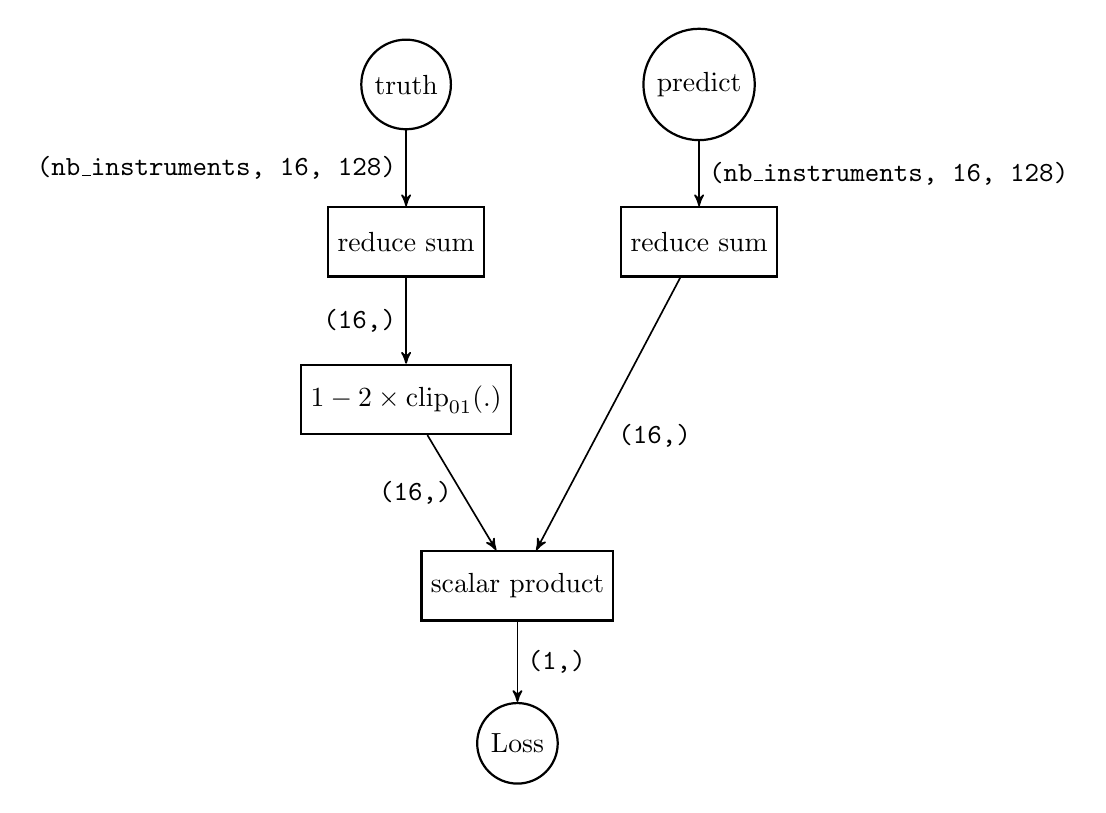
\begin{tikzpicture}[->, >=stealth', auto, semithick, node distance=2cm]
    \tikzstyle{every state}=[fill=white,draw=black,thick,text=black,scale=1]
    
    \node[state](truth)[left=1.cm]{ truth };
    \node[state](predict)[right of=truth, right=1.cm]{predict};
    
    \node[state, rectangle](t1)[below of=truth]{reduce sum};
    
    \node[state, rectangle](p1)[below of=predict]{reduce sum};
    
    \node[state, rectangle](t2)[below of=t1]{$1 - 2 \times \text{clip}_{01}(.)$};
    
    \node[state, rectangle](n1)[below right of=t2, below=0.5cm]{scalar product};
    
    \node[state](loss)[below of=n1]{Loss};
    
    
    \path[]
        (truth) edge    node[left]{\texttt{(nb\_instruments, 16, 128)}}   (t1)
        
        (predict)   edge    node{\texttt{(nb\_instruments, 16, 128)}}   (p1)
        
        (t1)    edge    node[left]{\texttt{(16,)}}    (t2)
        (t2)    edge    node[left]{\texttt{(16,)}}    (n1)
        (p1)    edge    node{\texttt{(16,)}}    (n1)
        (n1)    edge    node{\texttt{(1,)}} (loss);
        
    \end{tikzpicture}
\end{center}
\caption{Rhythm Loss}
\label{fig:loss_rhythm}
\end{figure}

\subsection{Harmony}

I explained in the section \ref{sec:harmonics} that some notes will sound smooth together because of their common harmonics.
On the other side, some notes won't be elegant when played together because of the resonance problem between some of their harmonics.

This is something every composer has in mind when he creates a second musical part which will harmonize the first one.
He will keep the second voice in the scale and he will keep an acceptable musical interval between the notes of the 2 melodic parts.

The figure \ref{fig:harmony_circle} shows the acceptable and non-acceptable musical intervals for the note $A$.

\begin{figure}[ht]
    \centering
    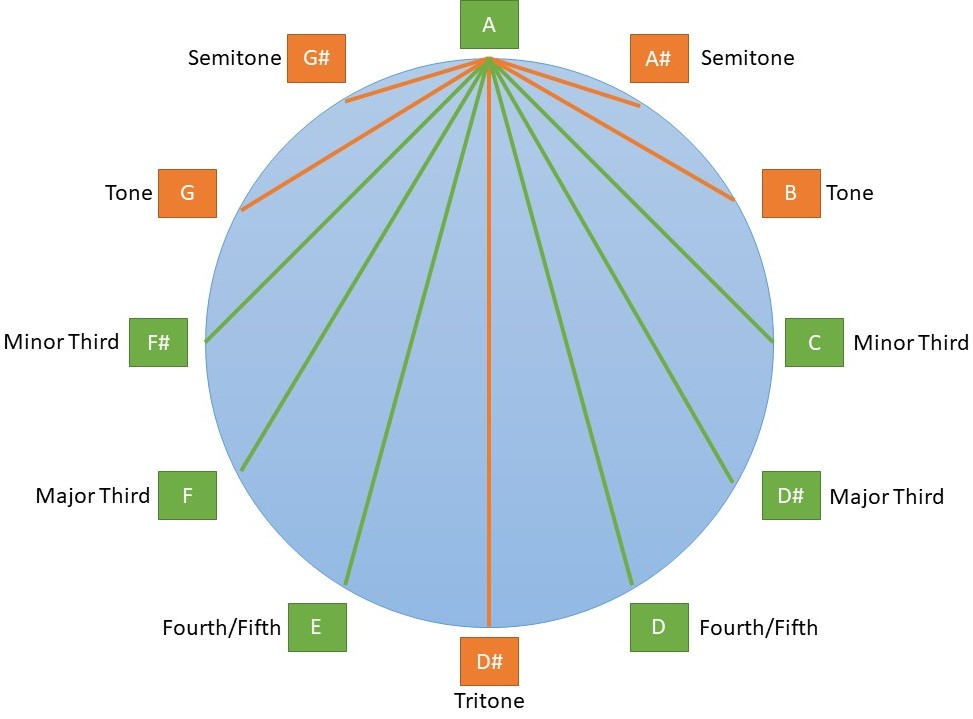
\includegraphics[width=\textwidth]{images/music/circle_harmony.jpg}
    \caption{Harmony Circle for $A$}
    \label{fig:harmony_circle}
\end{figure}

From this figure, I realized there are actually 3 musical intervals to avoid:
\begin{itemize}
    \item The \textit{semitone} interval
    \item The \textit{tone} interval
    \item The \textit{tritone} interval. Actually, this interval was named \textit{"Diabolus in musica"} ("Devil in the music") and was forbidden by the church.
\end{itemize}

To prevent the model to generate such intervals, I created a loss function which gives a penalty every time there is one of this intervals.
To do so, I created a sub-function $\text{harmony}_n$ which penalizes the presence of the $n^{th}$ interval (counted in semitone).

The operations of the cost function harmony and $\text{harmony}_n$ are showed in the figures \ref{fig:loss_harmony} and \ref{fig:loss_harmony_n}.
The $\text{roll}_n$ operation is explained in the appendix \ref{appendix:roll_n}.


\begin{figure}[H]
    \begin{minipage}{0.5\textwidth}
        \begin{center}
            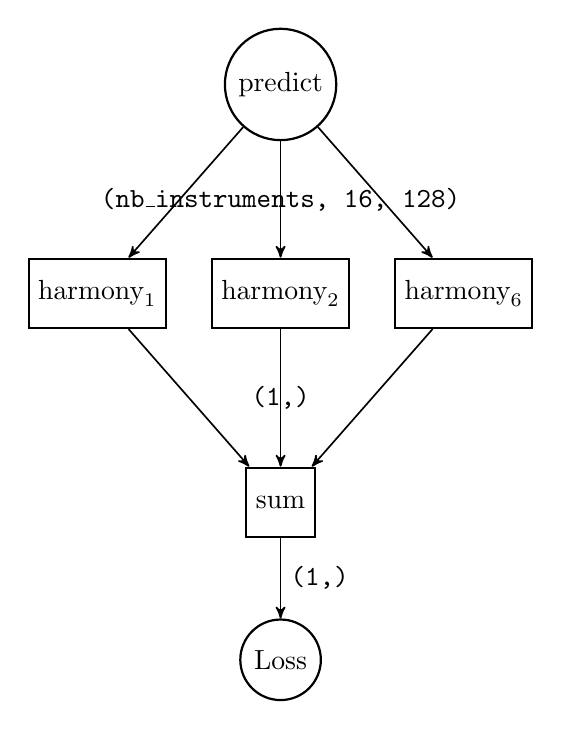
\begin{tikzpicture}[->, >=stealth', auto, semithick, node distance=2cm]
            \tikzstyle{every state}=[fill=white,draw=black,thick,text=black,scale=1]
            
            \node[state](n0)[]{predict};
            \node[](nleft)[left of=n0, left=0.2cm]{};
            \node[](nrigth)[right of=n0, right=0.2cm]{};
            
            
            \node[state, rectangle](h1)[below of=nleft, below=0.2cm]{$\text{harmony}_1$};
            \node[state, rectangle](h2)[below of=n0, below=0.2cm]{$\text{harmony}_2$};
            \node[state, rectangle](h6)[below of=nrigth, below=0.2cm]{$\text{harmony}_6$};
            
            \node[state, rectangle](s)[below of=h2, below=0.2cm]{sum};
            
            \node[state](loss)[below of=s]{Loss};
            
            \path[]
                (n0)    edge    node{}  (h1)
                        edge    node[anchor=center]{\texttt{(nb\_instruments, 16, 128)}}   (h2)
                        edge    node{}  (h6)
                (h1)    edge    node{}  (s)
                (h2)    edge    node[anchor=center]{\texttt{(1,)}}  (s)
                (h6)    edge    node{}  (s)
                (s)     edge    node{\texttt{(1,)}} (loss);
                
            \end{tikzpicture}
        \end{center}
        \caption{Harmony Loss}
        \label{fig:loss_harmony}
    \end{minipage} \hfill
    \begin{minipage}{0.5\textwidth}
        \begin{center}
            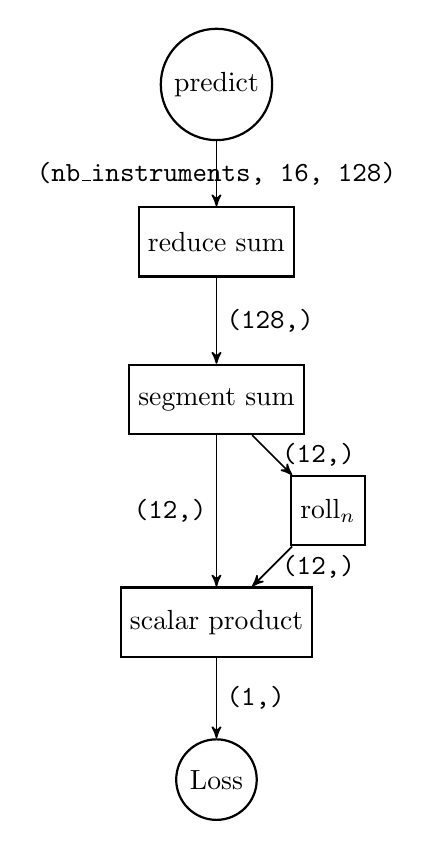
\begin{tikzpicture}[->, >=stealth', auto, semithick, node distance=2cm]
            \tikzstyle{every state}=[fill=white,draw=black,thick,text=black,scale=1]
            
            \node[state](predict)[]{predict};
            
            \node[state, rectangle](n1)[below of=predict]{reduce sum};
            \node[state, rectangle](n2)[below of=n1]{segment sum};
            
            \node[state, rectangle](r)[below right of=n2]{$\text{roll}_n$};
            
            \node[state, rectangle](s)[below left of=r]{scalar product};
            
            \node[state](loss)[below of=s]{Loss};
            
            
            \path[]
                (predict)   edge    node[anchor=center]{\texttt{(nb\_instruments, 16, 128)}}    (n1)
                (n1)    edge    node{\texttt{(128,)}}   (n2)
                (n2)    edge    node[right]{\texttt{(12,)}}    (r)
                        edge    node[left]{\texttt{(12,)}}  (s)
                (r)     edge    node[right]{\texttt{(12,)}} (s)
                (s)     edge    node{\texttt{(1,)}} (loss);
                
            \end{tikzpicture}
        \end{center}
        \caption{$\text{Harmony}_n$ Loss}
        \label{fig:loss_harmony_n}
    \end{minipage}
\end{figure}

% ----------------------------------------------------------------------------------------------------
% Experiments
% ----------------------------------------------------------------------------------------------------
\chapter{Experiments}

% ----------------------------------------------------------------------------------------------------
% Conclusion
% ----------------------------------------------------------------------------------------------------

\chapter{Conclusion}

This dissertation project provides a new neural network architecture (RMVAE) and a new layer to handle time dependencies between data (RPOE).

I have showed that the RMVAE architecture is able to learn musical rules from a pianoroll view and adding extra losses (Scale, Rhythm and Harmony losses) doesn't help the training.

% ----------------------------------------------------------------------------------------------------
% Future work
% ----------------------------------------------------------------------------------------------------

\section*{Future work}
Find the scale with some already known scale template ?

Try with different encoding : Text
BachBot or DeepBach says the way you write music with text is important 
Maybe convolution and image is not good enough

I constructed my own pianoroll view.
Maybe try to use Pypianoroll will give a better representation.


I didn't want to change the dataset to C major so it can handle change of key. But seems too hard for the neural network
\newpage

% ####################################################################################################
% ####################################################################################################
% Bibliography
% ####################################################################################################
% ####################################################################################################
\bibliographystyle{IEEEtran}
\bibliography{IEEEabrv, biblio/Dissertation.bib}
% \printbibliography

% ####################################################################################################
% ####################################################################################################
% Appendix
% ####################################################################################################
% ####################################################################################################

\newpage

\chapter*{Appendices}
\addcontentsline{toc}{chapter}{Appendices}      % To not display number of chapter in table of content
\appendix

\section{Interpolation project}

\section{Segment Sum}
\label{appendix:segment_sum}

The segment sum operation allows me to sum the values of a vector of shape \texttt{(128,)} (corresponding of all the different notes in the different octaves) in a vector of shape \texttt{(12,)} (corresponding to the different 12 notes).

The figure \ref{fig:segment_sum} describes what the segment sum operation would perform if there were only 4 different notes (\textit{A, B, C, D}) and 3 different octaves (\textit{1, 2, 3}) for a total of 12 notes.

\begin{figure}[ht]
    \centering
    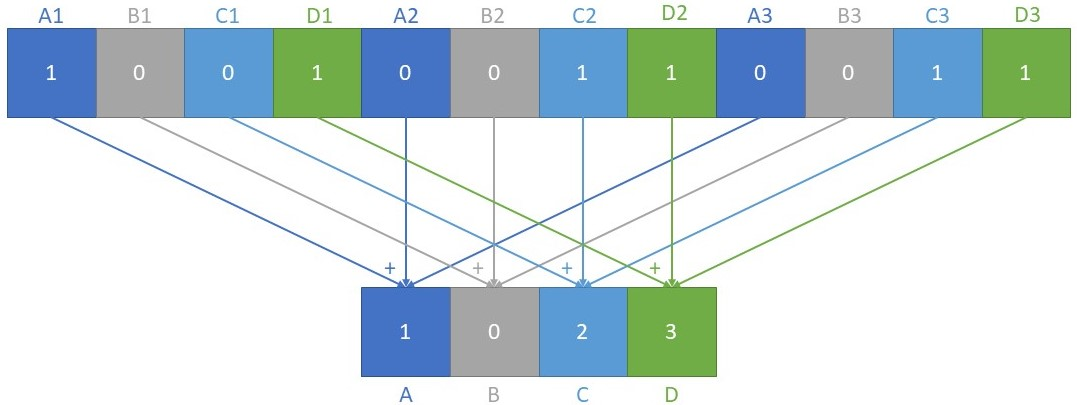
\includegraphics[width=\textwidth]{images/nn/tensor/segment_sum.jpg}
    \caption{Segment sum operation}
    \label{fig:segment_sum}
\end{figure}

\section{$\text{Roll}_n$}
\label{appendix:roll_n}

The $\text{Roll}_n$ operation takes a one dimensional tensor, takes the first $n$ values and put append them at the end.
The algorithm \ref{alg:roll_n} explains how it works and the figure \ref{fig:roll_2} shows an example with $n=2$.

\begin{algorithm}
    \begin{algorithmic}[1]
        \Require{tensor, n} 
        \Ensure{$tensor$ (Rolled tensor)}
        \Statex
        \Function{Roll}{$tensor, n$}
            \For{$k \gets 1$ to $n$}
                \State {$firstElement \gets tensor.pop(0)$}
                \State {$tensor.append(firstElement)$}
            \EndFor
            \State \Return {$tensor$}
        \EndFunction
        \end{algorithmic}
    \caption{$\text{Roll}_n$ function}
    \label{alg:roll_n}
\end{algorithm}

\begin{figure}[ht]
    \centering
    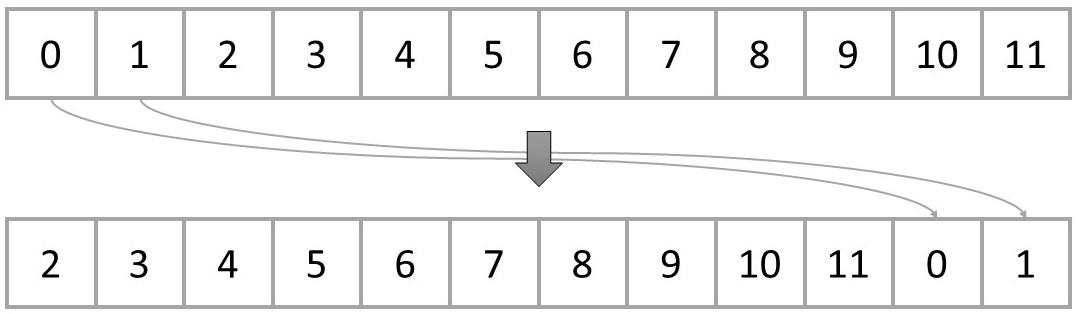
\includegraphics[width=\textwidth]{images/nn/tensor/roll_2.jpg}
    \caption{$\text{Roll}_2$ example}
    \label{fig:roll_2}
\end{figure}

\section{BandPlayer}

\section{Coconet Process}
\label{appendix:coconet_process}

The figure \ref{fig:coconet_process} illustrates the coconet process.
This process is explained in the section \ref{sec:rw:nade}.

\begin{figure}[htbp]
    \centering
    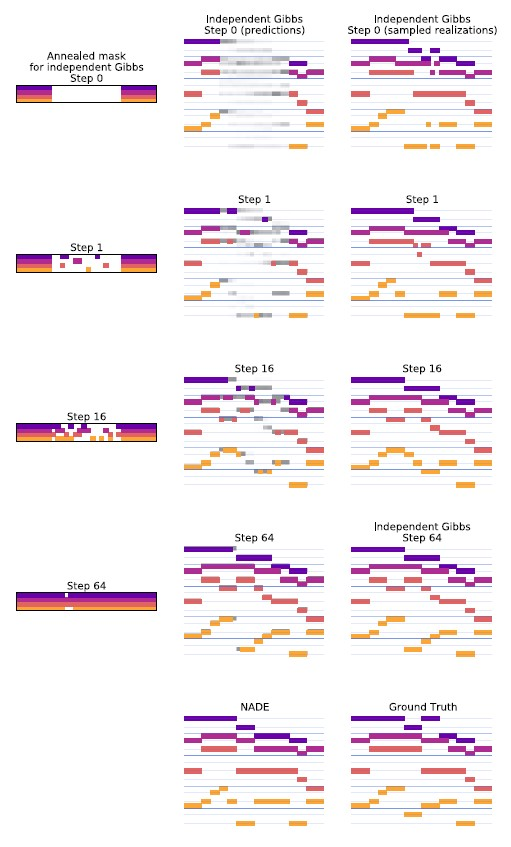
\includegraphics[width=0.8\textwidth]{images/related_works/coconet/coconet_process.jpg}
    \caption{COCONET process}
    Source: Cheng-Zhi Anna Huang et al.'s paper \cite{huang_counterpoint_2017}
    \label{fig:coconet_process}
\end{figure}

\section{Transformer architecture}

The figure \ref{fig:arch:transformer} illustrates the transformer's architecture. This architecture is explained in the section \ref{sec:back:transformers}.

\begin{figure}[htbp]
    \centering
    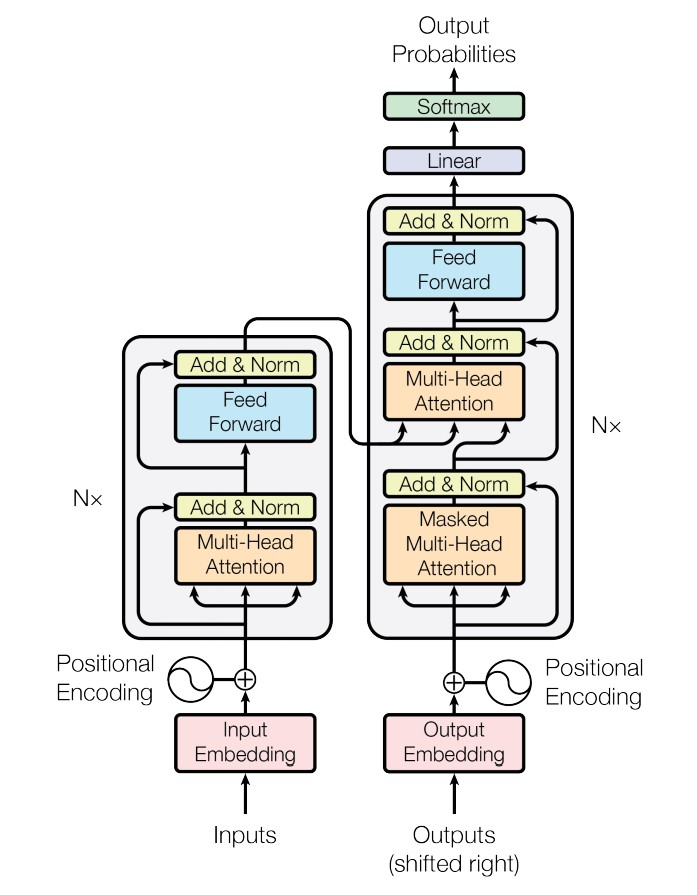
\includegraphics[width=\textwidth]{images/related_works/transformer/transformer_architecture.jpg}
    \caption{Transformer architecture}
    Source: Ashish Vaswani et al.'s paper \cite{vaswani_attention_2017-1}
    \label{fig:arch:transformer}
\end{figure}


\end{document}

% Photographs, Illustrations and Other Attachments
% [For soft-bound, paper copy for Examination/Re-examination] Photographic and other illustrations that are to be included in the bound copy of the thesis have to be securely mounted using double-faced tape. Photograph album pockets or slits in the page are not adequate. In no circumstances should ‘cellophane tape’ or a similar material be used for any purpose in a copy of the thesis. All copies of the thesis should contain original photographs. Subsidiary papers and other loose material should be bound in wherever possible. If this is not possible, an adequately guarded pocket for each material should be provided at the end of the thesis. Any such loose material (and corrigenda sheets, if not bound in) should bear the candidate’s name, initials and degree.
% Photographic and other illustrations (e.g. line drawings, maps, musical scores, etc.) which need to be uploaded in the ETD system should be inserted in the thesis in PDF format as far as possible.
